\section{Bound on bias in gradient descent}
\label{sec grad des bias}

We complete the analysis from Section~\ref{sec stoch alg for calibration} for a general loss function here.
\begin{theorem}\label{th bias}
Let Assumption \ref{ass diff payoff} hold. Consider the family of neural SDEs \eqref{eq:nsde}. We have 
\begin{equation}\label{eq bias 1}
\begin{split}
&\left|\EE[\partial_{\theta}h^{N}(\theta) ] - \partial_{\theta}h(\theta)\right| \\
& \qquad \leq \left( \EE\left[ \left(\partial_x \ell\left(\EE^{\QQ^N(\theta)}[\phi^{\textup{cv}}(X^{\theta})],\Pp(\Phi) \right)- \partial_x \ell\left(\EE^{\QQ}[\phi^{\textup{cv}}(X^{\theta})],\Pp(\Phi) \right) \right)^2 \right] \right)^{1/2} \\
& \hskip0.55\textwidth \times \left( \EE \left[\left(\EE^{\QQ^N(\theta)}[\partial_\theta \phi(X^{\theta})]\right)^2\right] \right)^{1/2}\,.
 \end{split}
\end{equation}
If in addition, we assume that the loss function~$\ell$ is three times differentiable in the  first variable with all derivatives of second and third-order bounded, then
\begin{small}
\begin{equation}\label{eq bias 2}
\begin{split}
 	&\left| \EE^{\QQ}\left[\partial_{\theta} h^{N}(\theta)\right] -  \partial_{\theta}h(\theta) \right|\\ 
 	 & \leq \frac{1}{2}  \bigg\{ \| \partial_x^3 \ell\|_{\infty}  \left\lvert \EE^{\QQ}[\partial_\theta \phi(X^{\theta})]\right\rvert 
 \frac{1}{N}\Var^{\QQ}[\phi^{\textup{cv}}(X^{\theta})] \\
 	 & + \| \partial_x^3 \ell\|_{\infty}
 	  \left( \frac{1}{N}\Var^{\QQ}[\partial_\theta \phi(X^{\theta})]\right)^{1/2}
 	   \left( \frac{1}{N^3} \EE[(\phi^{\textup{cv}}(X^{\theta}) - \EE^{\QQ}[\phi^{\textup{cv}}(X^{\theta})])^4]  +  \frac{3}{N^2} (\Var^{\QQ}[\phi^{\textup{cv}}(X^{\theta})])^2\right)^{1/2} \\
 & + 2 \| \partial_x^2 \ell\|_{\infty}  \left( \frac{1}{N} \Var^{\QQ}[\partial_{\theta}\phi(X^{\theta})]   \right)^{1/2}\left( \frac{1}{N} \Var^{\QQ}[\phi^{\textup{cv}}(X^{\theta})] \right)^{1/2}\bigg\}\,.
 \end{split}
\end{equation}
\end{small}%
\end{theorem}
\begin{proof}
Observe that
\[
\EE \left[\EE^{\QQ^N}[\phi^{\textup{cv}}(X^{\theta})]\right] = \EE^{\QQ}[\phi^{\textup{cv}}(X^{\theta})] \quad \text{and} \quad \EE \left[ \EE^{\QQ^N}[\partial_\theta \phi(X^{\theta})] \right] =\EE^{\QQ}[\partial_\theta \phi(X^{\theta})]\,.
\]  
The second equality implies that
\[
 \EE\left[ \partial_x \ell\left(\EE^{\QQ}[\phi^{\textup{cv}}(X^{\theta})],\Pp(\Phi) \right) \EE^{\QQ^N}\left[\partial_\theta \phi(X^{\theta})\right] \right] =
  \partial_{\theta}h(\theta)\,.
\]
Next, by adding and subtracting~$\partial_x \ell(\EE^{\QQ}[\phi^{\textup{cv}}(X^{\theta})],\Pp(\Phi) )$ and using above observation along with the Cauchy--Schwarz inequality we have
\[
\begin{split}
& | \EE[\partial_{\theta}h^{N}(\theta) ] - \partial_{\theta}h(\theta) |\\
	& =  \left| \EE\left[\left(\partial_x \ell\left(\EE^{\QQ^N}[\phi^{\textup{cv}}(X^{\theta})],\Pp(\Phi) \right) + \partial_x \ell\left(\EE^{\QQ}[\phi^{\textup{cv}}(X^{\theta})],\Pp(\Phi) \right) -\partial_x \ell\left(\EE^{\QQ}[\phi^{\textup{cv}}(X^{\theta})],\Pp(\Phi) \right) \right) \right.\right. \\ & \qquad \qquad \left.\left. \times \; \EE^{\QQ^N}\left[\partial_\theta \phi(X^{\theta})\right]\right]
 - \partial_{\theta}h(\theta) \right|\, \\
& = \left|\EE\left[\left(\partial_x \ell\left(\EE^{\QQ^N}[\phi^{\textup{cv}}(X^{\theta})],\Pp(\Phi) \right)- \partial_x \ell\left(\EE^{\QQ}[\phi^{\textup{cv}}(X^{\theta})],\Pp(\Phi) \right) \right)\EE^{\QQ^N}\left[\partial_\theta \phi(X^{\theta})\right] \right]  \right| \,.
 \end{split}
\]
Hence
\begin{small}
\begin{equation*}
\begin{split}
& \left\lvert \EE[\partial_{\theta}h^{N}(\theta) ] - \partial_{\theta}h(\theta) \right\rvert\\
 & \leq \left( \EE\left[ \left(\partial_x \ell\left(\EE^{\QQ^N}[\phi^{\textup{cv}}(X^{\theta})],\Pp(\Phi) \right)- \partial_x \ell\left(\EE^{\QQ}[\phi^{\textup{cv}}(X^{\theta})],\Pp(\Phi) \right) \right)^2 \right] \right)^{1/2} \left( \EE \left[\EE^{\QQ^N}[\partial_\theta \phi(X^{\theta})]\right]^2 \right)^{1/2}\,.
 \end{split}
\end{equation*}
\end{small}%
This concludes the proof of \eqref{eq bias 1}. To prove \eqref{eq bias 2}, we view~$\partial_{\theta}h^{N}(\theta)$ as function of~$\big(\EE^{\QQ^N}[\phi^{\textup{cv}}(X^{\theta})], \allowbreak \EE^{\QQ^N}[\partial_\theta \phi(X^{\theta})]\big)$ and expand into its Taylor series around~$\big(\EE^{\QQ}[\phi^{\textup{cv}}(X^{\theta})], \EE^{\QQ}[\partial_\theta \phi(X^{\theta})]\big)$, i.e.,
\begin{small}
\begin{equation*}
\begin{split}
 	&\partial_{\theta}h^{N}(\theta) =  \partial_{\theta}h(\theta) \\ 
 	& + \partial_x^2 \ell\left(\EE^{\QQ}[\phi^{\textup{cv}}(X^{\theta})],\Pp(\Phi) \right) \EE^{\QQ}[\partial_\theta \phi(X^{\theta})]\left(\EE^{\QQ^N}[\phi^{\textup{cv}}(X^{\theta})]  - \EE^{\QQ}[\phi^{\textup{cv}}(X^{\theta})]  \right)  \\
        & + \partial_x \ell\left(\EE^{\QQ}[\phi^{\textup{cv}}(X^{\theta})],\Pp(\Phi) \right) \left( \EE^{\QQ^N}[\partial_\theta \phi(X^{\theta})]  - \EE^{\QQ}[\partial_\theta \phi(X^{\theta})]  \right) \\
        & + \frac{1}{2} \int_{0}^1 \Big\{\partial_x^3 \ell\left(\xi_1^{\alpha},\Pp(\Phi) \right) \xi_2^{\alpha}\left(\EE^{\QQ^N}[\phi^{\textup{cv}}(X^{\theta})]  - \EE^{\QQ}[\phi^{\textup{cv}}(X^{\theta})]  \right)^2 \\
        & \qquad + 2 \partial_x^2 \ell\left(\xi_1^{\alpha},\Pp(\Phi) \right) \left(\EE^{\QQ^N}[\partial_{\theta}\phi(X^{\theta})]  - \EE^{\QQ}[\partial_{\theta}\phi(X^{\theta})]  \right) \left(\EE^{\QQ^N}[\phi^{\textup{cv}}(X^{\theta})]  - \EE^{\QQ}[\phi^{\textup{cv}}(X^{\theta})]  \right)\Big\} \D\alpha\,,
\end{split}
\end{equation*}
\end{small}%
where for~$\alpha\in(0,1)$
 \[
 \begin{split}
 \xi_1^{\alpha} = &  \EE^{\QQ}[\phi^{\textup{cv}}(X^{\theta})]  + \alpha \left(
 \EE^{\QQ^N}[\phi^{\textup{cv}}(X^{\theta})] - \EE^{\QQ}[\phi^{\textup{cv}}(X^{\theta})] \right)\,, \\ 
  \xi_2^{\alpha} = &  \EE^{\QQ}[\partial_\theta \phi(X^{\theta})] + \alpha \left( \EE^{\QQ^N}[\partial_\theta \phi(X^{\theta})] - \EE^{\QQ}[\partial_\theta \phi(X^{\theta})] \right)\,.
 \end{split}
 \]
 Hence, using the Cauchy-Schwarz inequality 
 \[
 \begin{split}
 	&\left| \EE^{\QQ}\left[\partial_{\theta} h^{N}(\theta)\right] -  \partial_{\theta}h(\theta) \right|\\ 
 	 & \leq \frac{1}{2} \int_{0}^1 \EE \Big[ \Big\{ \| \partial_x^3 \ell\|_{\infty} \left| \EE^{\QQ}[\partial_\theta \phi(X^{\theta})]\right| \left(\EE^{\QQ^N}[\phi^{\textup{cv}}(X^{\theta})]  - \EE^{\QQ}[\phi^{\textup{cv}}(X^{\theta})]  \right)^2 \\
 	 & + \alpha\| \partial_x^3 \ell\|_{\infty}
 	 \left| \EE^{\QQ^N}[\partial_\theta \phi(X^{\theta})] - \EE^{\QQ}[\partial_\theta \phi(X^{\theta})] \right|
 	   \left(\EE^{\QQ^N}[\phi^{\textup{cv}}(X^{\theta})]  - \EE^{\QQ}[\phi^{\textup{cv}}(X^{\theta})]  \right)^2 \\
 & + 2 \| \partial_x^2 \ell\|_{\infty}  \left| \EE^{\QQ^N}[\partial_{\theta}\phi(X^{\theta})]  - \EE^{\QQ}[\partial_{\theta}\phi(X^{\theta})]  \right|\left|\EE^{\QQ^N}[\phi^{\textup{cv}}(X^{\theta})]  - \EE^{\QQ}[\phi^{\textup{cv}}(X^{\theta})] \right|\Big\} \Big]\D\alpha\,
 \end{split}
 \]
and
 \[
 \begin{split}
 &\left| \EE^{\QQ}\left[\partial_{\theta} h^{N}(\theta)\right] -  \partial_{\theta}h(\theta) \right| \leq \frac{1}{2}  \Bigg\{ \| \partial_x^3 \ell\|_{\infty}  \left| \EE^{\QQ}[\partial_\theta \phi(X^{\theta})]\right|
 \frac{1}{N}\Var^{\QQ}[\phi^{\textup{cv}}(X^{\theta})] \\
 	 & + \| \partial_x^3 \ell\|_{\infty}
 	  \left( \frac{1}{N}\Var^{\QQ}[\partial_\theta \phi(X^{\theta})]\right)^{1/2}
 	   \left( \EE \left[ \left(\EE^{\QQ^N}[\phi^{\textup{cv}}(X^{\theta})]  - \EE^{\QQ}[\phi^{\textup{cv}}(X^{\theta})]  \right)^4 \right] \right)^{1/2} \\
 & + 2 \| \partial_x^2 \ell\|_{\infty}  \left( \frac{1}{N} \Var ^{\QQ}[\partial_{\theta}\phi(X^{\theta})]   \right)^{1/2}\left( \frac{1}{N} \Var ^{\QQ}[\phi^{\textup{cv}}(X^{\theta})] \right)^{1/2}\Bigg\}\,.
 \end{split}
 \]
Now let ~$\lambda^i\defEqual \phi^{\textup{cv}}(X^{\theta,i}) - \EE^{\QQ}[\phi^{\textup{cv}}(X^{\theta})]~$, and note that
 \[
 \begin{split}
\left( \sum_{i=1}^N \lambda^i \right)^4 
 =& \sum_{i=1}^N (\lambda^i )^4 + 3 \sum_{i_1\neq i_2}^N (\lambda^{i_1} )^2 (\lambda^{i_2} )^2
+ 4 \sum_{i_1\neq i_2 }^N (\lambda^{i_1} )^1 (\lambda^{i_2} )^3 \\
&+ 6 \sum_{i_1, i_2, i_3\,\,\,  \text{distinct} }^N \lambda^{i_1} \lambda^{i_2} (\lambda^{i_3} )^2
+ \sum_{i_1, i_2, i_3,i_4 \,\,\,\text{distinct} }^N \lambda^{i_1} \lambda^{i_2}\lambda^{i_3}\lambda^{i_4}\,. 
\end{split}
 \]
Hence
\begin{align*}
&\EE \left[ \left(\EE^{\QQ^N}[\phi^{\textup{cv}}(X^{\theta})]  - \EE^{\QQ}[\phi^{\textup{cv}}(X^{\theta})]  \right)^4 \right] \\
&\qquad = \frac{1}{N^3} \EE\left[(\phi^{\textup{cv}}(X^{\theta}) - \EE^{\QQ}[\phi^{\textup{cv}}(X^{\theta})])^4\right]  +  \frac{3}{N^2} \left(\Var ^{\QQ}[\phi^{\textup{cv}}(X^{\theta})]\right)^2\,. 
\end{align*}
The proof is complete.  
\end{proof}


\section{Additional results of calibration to market data}\label{apx:calibration market data}
In this section, we include additional figures displaying the neural SDE fit to market data when targeting the SPX option prices and minimising (Figures~\ref{fig:SPX LSV calibration iv lower bound exotic},~\ref{fig:SPX LSV calibration iv error lower bound exotic}) or maximising the exotic option price (Figures~\ref{fig:SPX LSV calibration iv upper bound exotic},~\ref{fig:SPX LSV calibration iv error upper bound exotic}). 

\begin{figure}[H]
  \centering 
	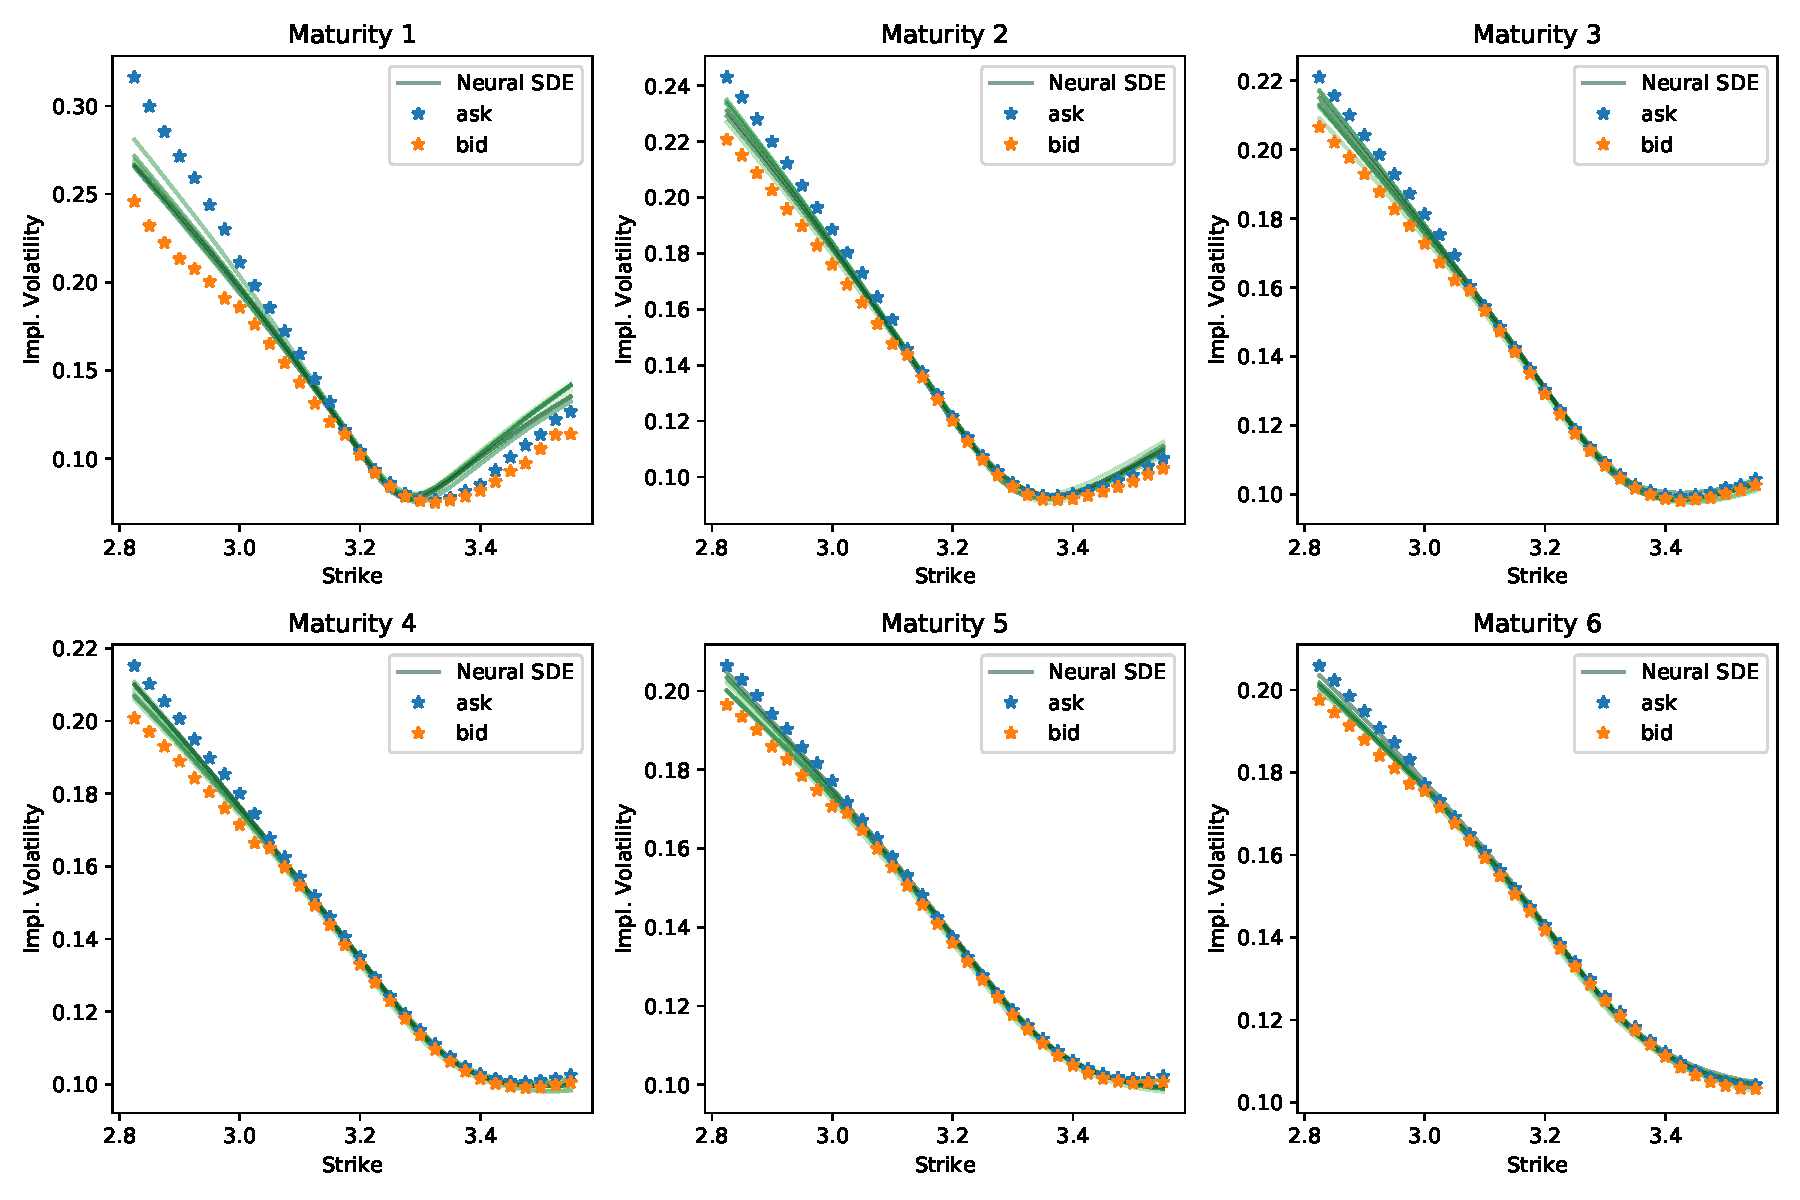
\includegraphics[clip, width=0.7\textwidth]{content/reschap1/Figures/figures_SPX/iv_nsde_lower_bound.pdf}
  \caption{Comparing market implied volatility and model implied volatility for the neural SDE LSV model~\eqref{eq:LSV_SDE} when targeting the {\em market data} and minimising the exotic option price.
We see implied volatility curves of the 10 calibrated neural SDEs vs. the market bid-ask spread for different maturities.
}
\label{fig:SPX LSV calibration iv lower bound exotic}  
\end{figure}


\begin{figure}[H]
  \centering 
	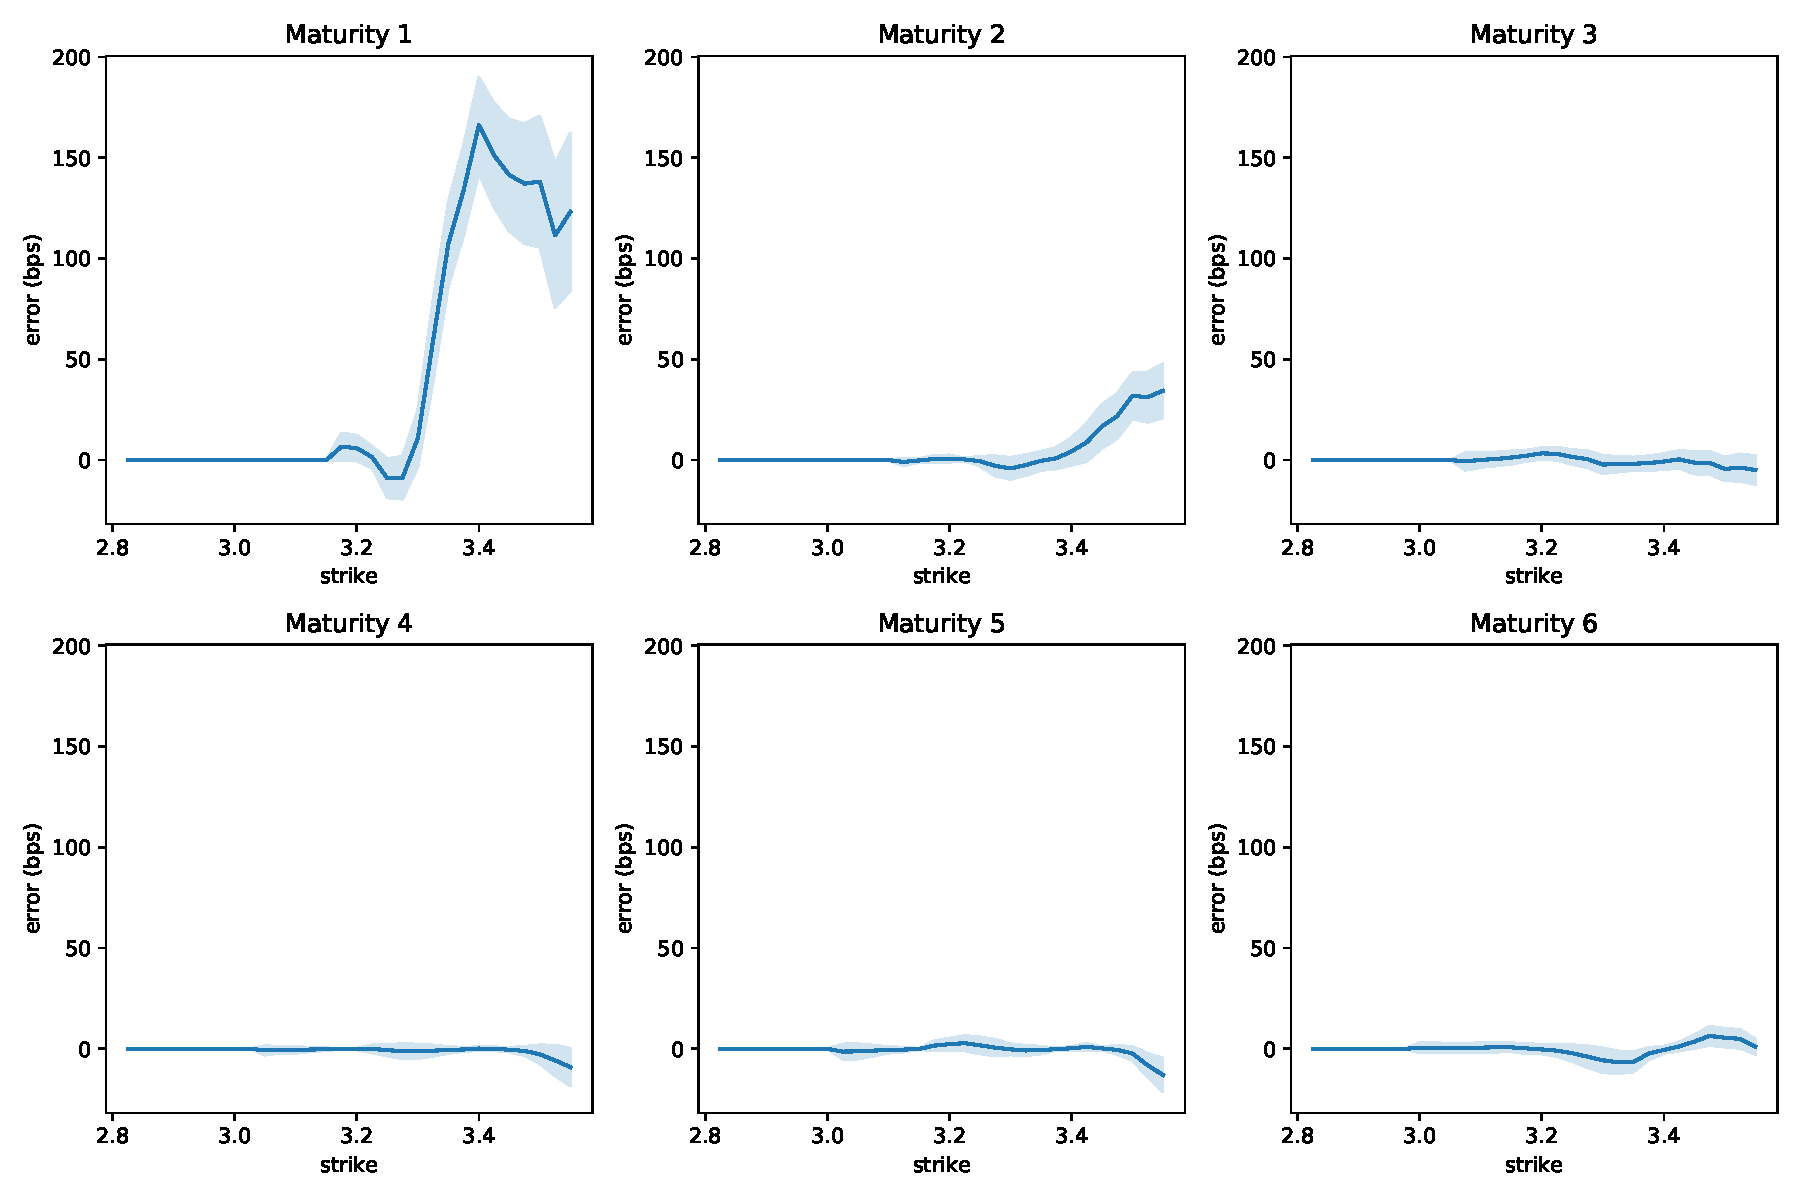
\includegraphics[clip, width=0.66\textwidth]{content/reschap1/Figures/figures_SPX/iv_error_lower_bound.pdf}
  \caption{Average error and standard deviation in basis points (bps) of the implied volatility curves from Figure~\ref{fig:SPX LSV calibration iv lower bound exotic}. The error is considered to be zero if the implied volatility falls into the bid-ask spread.
}
\label{fig:SPX LSV calibration iv error lower bound exotic}  
\end{figure}


\begin{figure}[H]
  \centering 
	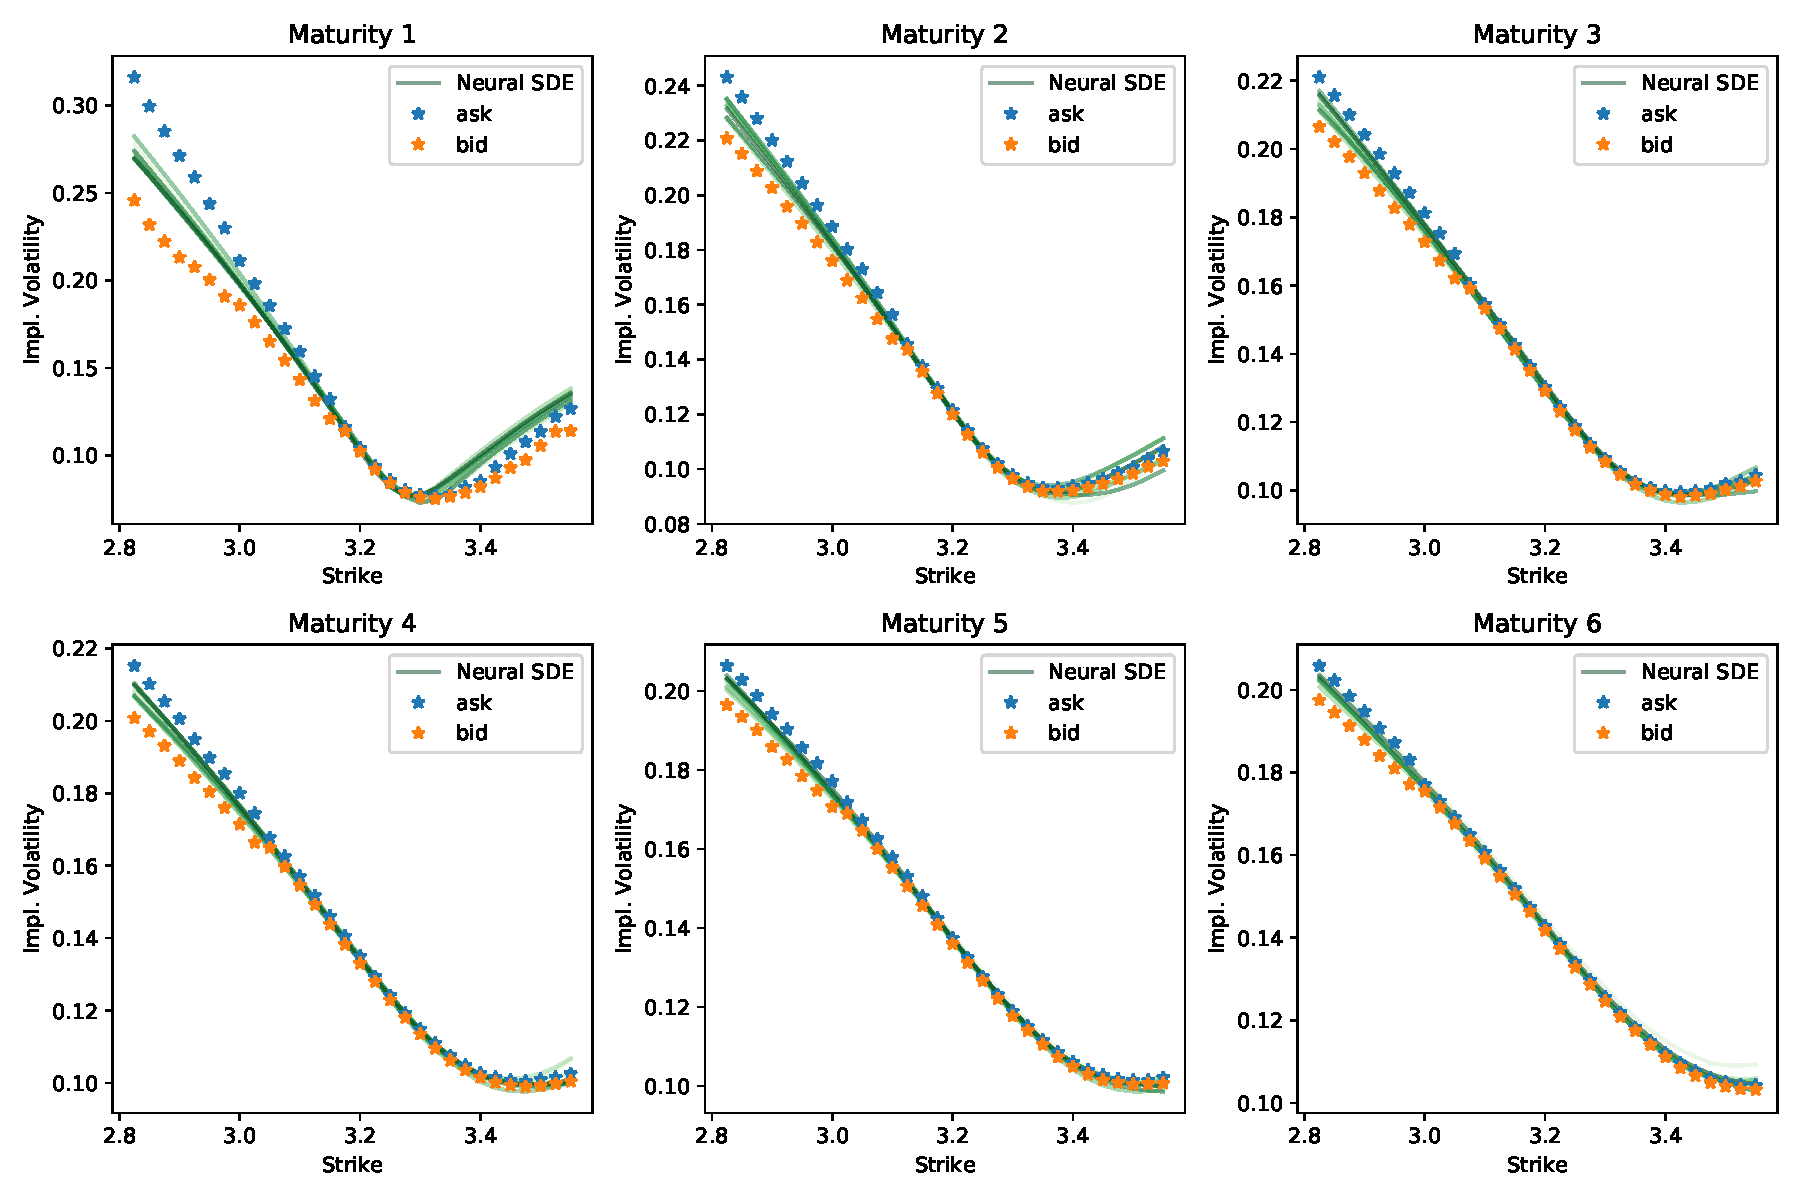
\includegraphics[clip, width=0.7\textwidth]{content/reschap1/Figures/figures_SPX/iv_nsde_upper_bound.pdf}
  \caption{Comparing market implied volatility and model implied volatility for the neural SDE LSV model~\eqref{eq:LSV_SDE} when targeting the {\em market data} and maximising the exotic option price.
We see implied volatility curves of the 10 calibrated neural SDEs vs. the market bid-ask spread for different maturities.
}
\label{fig:SPX LSV calibration iv upper bound exotic}  
\end{figure}


\begin{figure}[H]
  \centering 
	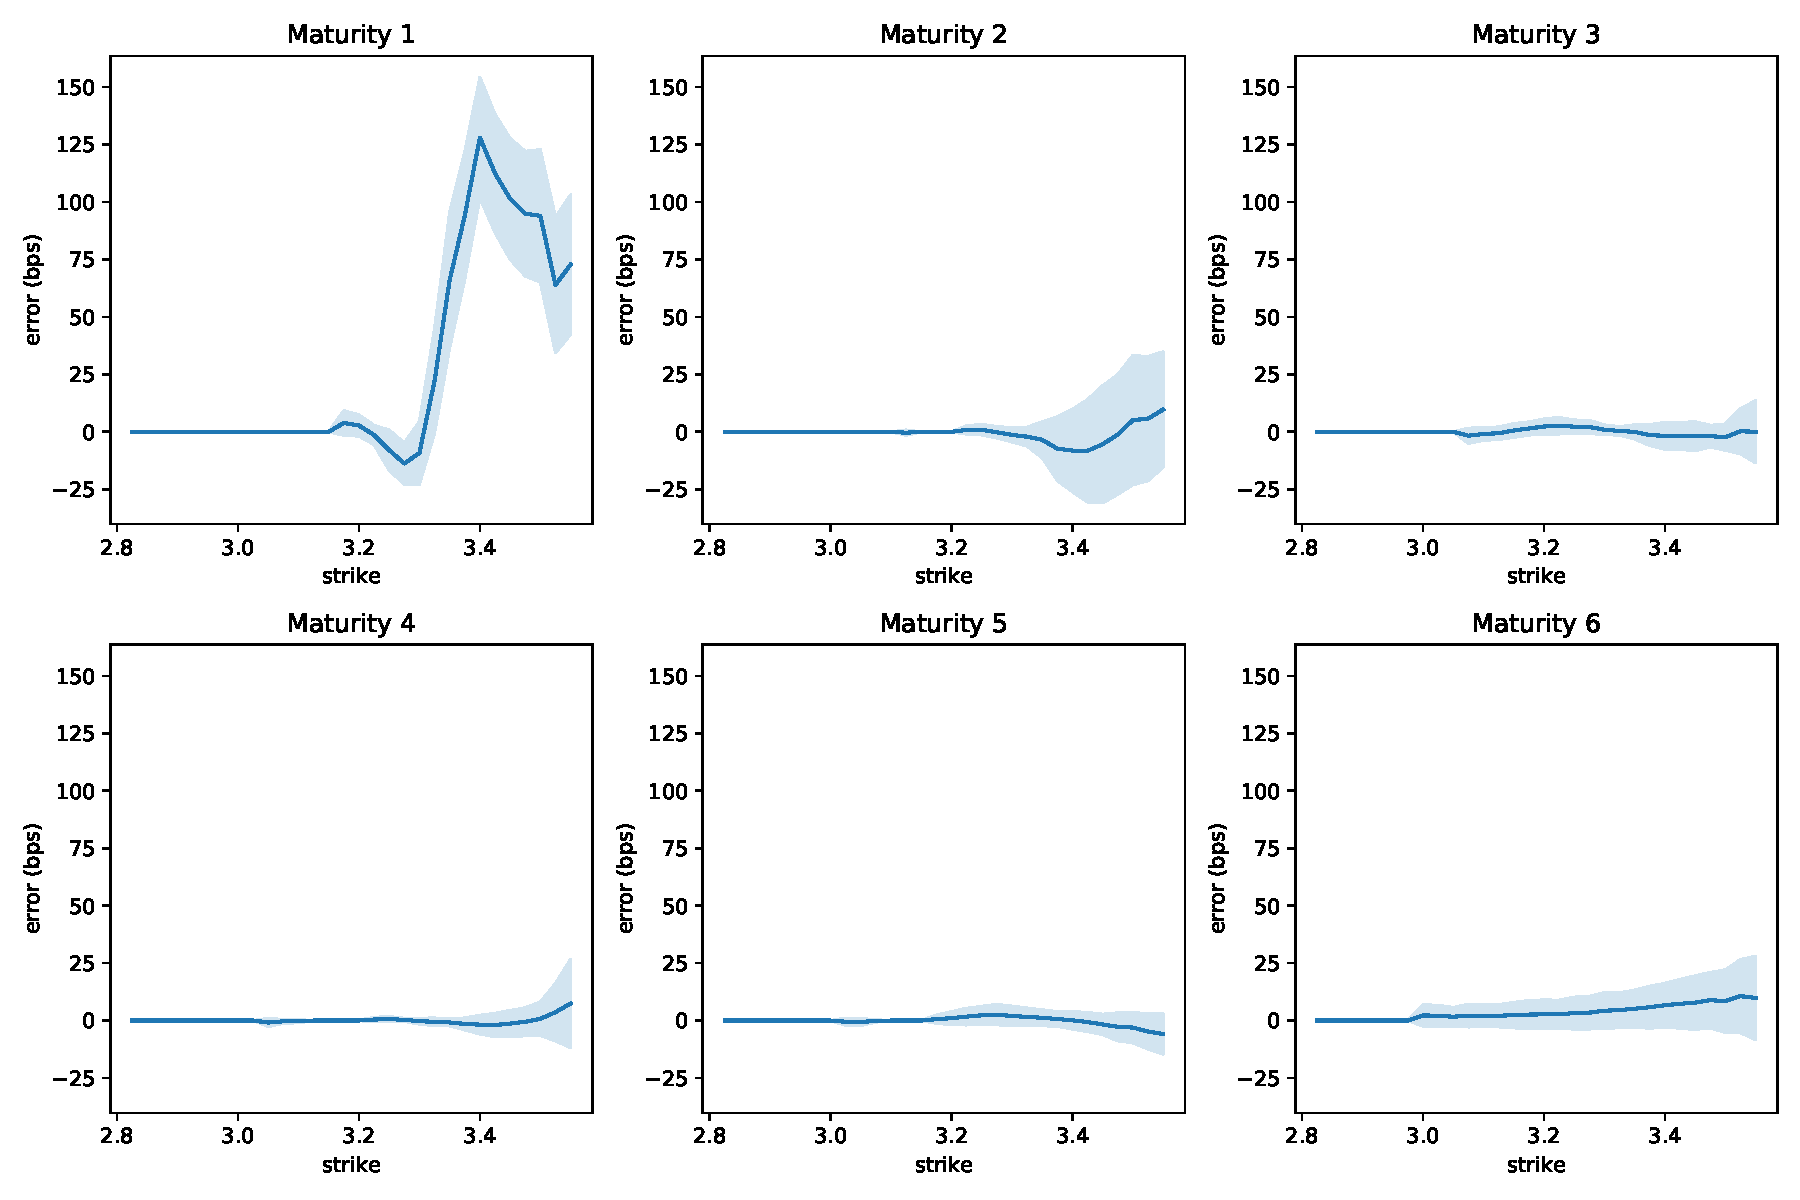
\includegraphics[clip, width=0.66\textwidth]{content/reschap1/Figures/figures_SPX/iv_error_upper_bound.pdf}
  \caption{Average error and standard deviation in basis points (bps) of the implied volatility curves from Figure~\ref{fig:SPX LSV calibration iv upper bound exotic}. The error is considered to be zero if the implied volatility falls into the bid-ask spread. 
}
\label{fig:SPX LSV calibration iv error upper bound exotic}  
\end{figure}



%\section{Calibration to Synthetic data}\label{sec:calibration synthetic data}
%
%
%In this experiment, we calibrate to European option prices
%\[
%\Pp(\Phi) \defEqual \EE^{\QQ(\theta)}[\Phi] = e^{-rT} \EE^{\QQ} \left[\left(S_T^\theta - K \right)_+ \middle\vert \, S_0 = 1\right]
%\]
%for maturities of~$2,4,\ldots,12$ months and~$21$ uniformly spaced strikes between in~$[0.8, 1.2]$. 
%As an example of an illiquid derivative for which we wish to find robust bounds we take the lookback option
%\[
%\Pp(\Psi) \defEqual \EE^{\QQ(\theta)}[\Psi] = e^{-rT} \EE^{\QQ} \left[\max_{t\in[0,T]}S_t^\theta - S_T \middle\vert \, S_0 = 1 \right]\, .
%\]
%The asset price~$S_t$ is generated using the Heston model described in Appendix~\ref{CalData}. We consider the same setting as in Section~\ref{sec numerics} and additionally also fit a Local volatility neural SDE model. 
%
%\subsection{Local volatility neural SDE model}
%\label{sec:LVintro}
%In this section we consider a Local Volatility (LV) neural SDE model.
%It has been shown by~\cite{dupire1994pricing} (see also~\cite{gyongy1986mimicking}) that if the data consisted of a continuum of call / put prices for all strikes and maturities, then there is a unique function~$\sigma$ such that with the price process
%\begin{align}\label{LV}
%  \D S_t = rS_t\,\D t + S_t \, \sigma(t,S_t)\D W_t\,,\,\,\,S_0=1\,
%\end{align}
%the model prices and market prices match exactly. 
%In practice only some calls / put prices are liquid in the market and so to apply~\cite{dupire1994pricing} one has to interpolate, in an arbitrage-free way, the missing data. 
%The choice of interpolation method is a further modelling choice on top of the one already made by postulating that the risky asset evolution is governed by~\eqref{LV}.   
%
%We will use a neural SDE instead of directly interpolating the missing data. 
%Let our LV neural SDE model be given by
%\begin{equation}\label{NeuralLV}
%\D S_t^\theta=rS_t^\theta\D t+\sigma(t,S_t^\theta, \theta)S_t^\theta \D W_t^{\QQ},
%\end{equation}
%where~$S_t^\theta \geq 0$,~$S_0^\theta=1$ and~$\sigma:[0,T]\times \RR \times \RR^q \to \RR^+$ allows us to calibrate the model to observed market prices.
%
%\subsection{Local stochastic volatility neural SDE model} 
%\label{sec LSV}
%
%In this section we consider a Local Stochastic Volatility (LSV) neural SDE model.
%See, for example,~\cite{tian2015calibrating}.
%As in the Local Volatility neural SDE model~\eqref{NeuralLV}, we have the risky asset price price process~$(S_t)_{t\in[0,T]}$, where the drift is equal to the risk-free bond rate~$r$. 
%However, the volatility function in the LSV neural SDE model
%now depends on~$t$,~$S_t$ and a stochastic process~$(V_t)_{t\in[0,T]}$.
%Here~$(V_t)_{t\in[0,T]}$ is not a traded asset.
%The model is then given by
%\begin{equation}\label{eq LSV SDE}
%\begin{split}
%\D S_t & = r S_t\D t + \sigma^S(t,S_t, V_t, \nu)S_t \,dB^S_t, \quad S_0 = 1,\\
%dV_t & = b^V(V_t, \phi)\,\D t + \sigma^V(V_t, \varphi) \,dB^V_t, \quad V_0 = v_0, \\
%d\langle B^S, B^V\rangle_t & = \rho\D t 
%\end{split}
%\end{equation}
%where 
%$\theta \defEqual \{\nu, \phi, \varphi, v_0, \rho \},\,\,\rho\in[-1,1], \,v_0>0, 
%$
%as the set of (multi-dimensional) parameters that we aim to optimise so that 
%the model is calibrated to the observed market data. 


%\subsection{Deep learning setting for the LV and LSV neural SDE models}
%In the SDE~\eqref{NeuralLV} the function~$\sigma$ and the SDE~\eqref{eq LSV SDE} the functions~$\sigma^S$,~$b^V$ and~$\sigma^V$ are parametrised by one feed-forward neural 
%network per maturity (see Section~\ref{sec many maturities} and Appendix~\ref{FFNNs}) with~$4$ hidden layers with~$50$ neurons in each layer. 
%The non-linear activation
%function used in each of the hidden layers is the linear rectifier \texttt{relu}. In addition, in~$\sigma^S$ and~$\sigma^V$
%after the output layer we apply the non-linear rectifier \texttt{softplus}$(x)=\log(1+\exp(x))$ to ensure a positive output. 
%
%The parameterisation of the hedging strategy for the vanilla option prices is also a feed-forward
%linear network with 3 hidden layers, 20 neurons per hidden layer and \texttt{relu} activation functions. 
%However, to get one hedging strategy per vanilla option 
%considered in the market data, the output of~$\mathfrak{h}(t_k, s_{t_k, \theta}^{i}, \xi_{K_j})$ has as many neurons as strikes and maturities.
%
%Finally, the parameterisation of the hedging strategy for the exotic options price is also a feed-forward
%network with 3 hidden layers, 20 neurons per hidden layer and \texttt{relu} activation functions.
%
%The neural SDEs~\eqref{NeuralLV} and~\eqref{eq LSV SDE} were discretized using the tamed Euler scheme~\eqref{eq tamed scheme} with~$N_{\text{steps}} = 8 \times 12$ uniform time steps for~$T=1$ year (i.e.~$16$ for every~$2$ months). 
%The number of Monte Carlo trajectories in each stochastic gradient descent iteration was~$N=4\times 10^4$ and the abstract hedging strategy was used as a control variate.
%
%Finally in the evaluation of the calibrated neural SDE, the option prices are calculated using~$N = 4\times 10^5$ trajectories of the calibrated neural SDEs, which we generated with~$2\times 10^5$ Brownian paths and their antithetic paths; in addition, we also used the learned hedging strategies to calculate the Monte Carlo estimators with lower variance~$\EE^{\QQ(\theta)}[\Phi_i^{\textup{cv}}]$ and~$\EE^{\QQ(\theta)}[\Psi^{\textup{cv}}]$.          


%\begin{figure}[h]
%\centering 
%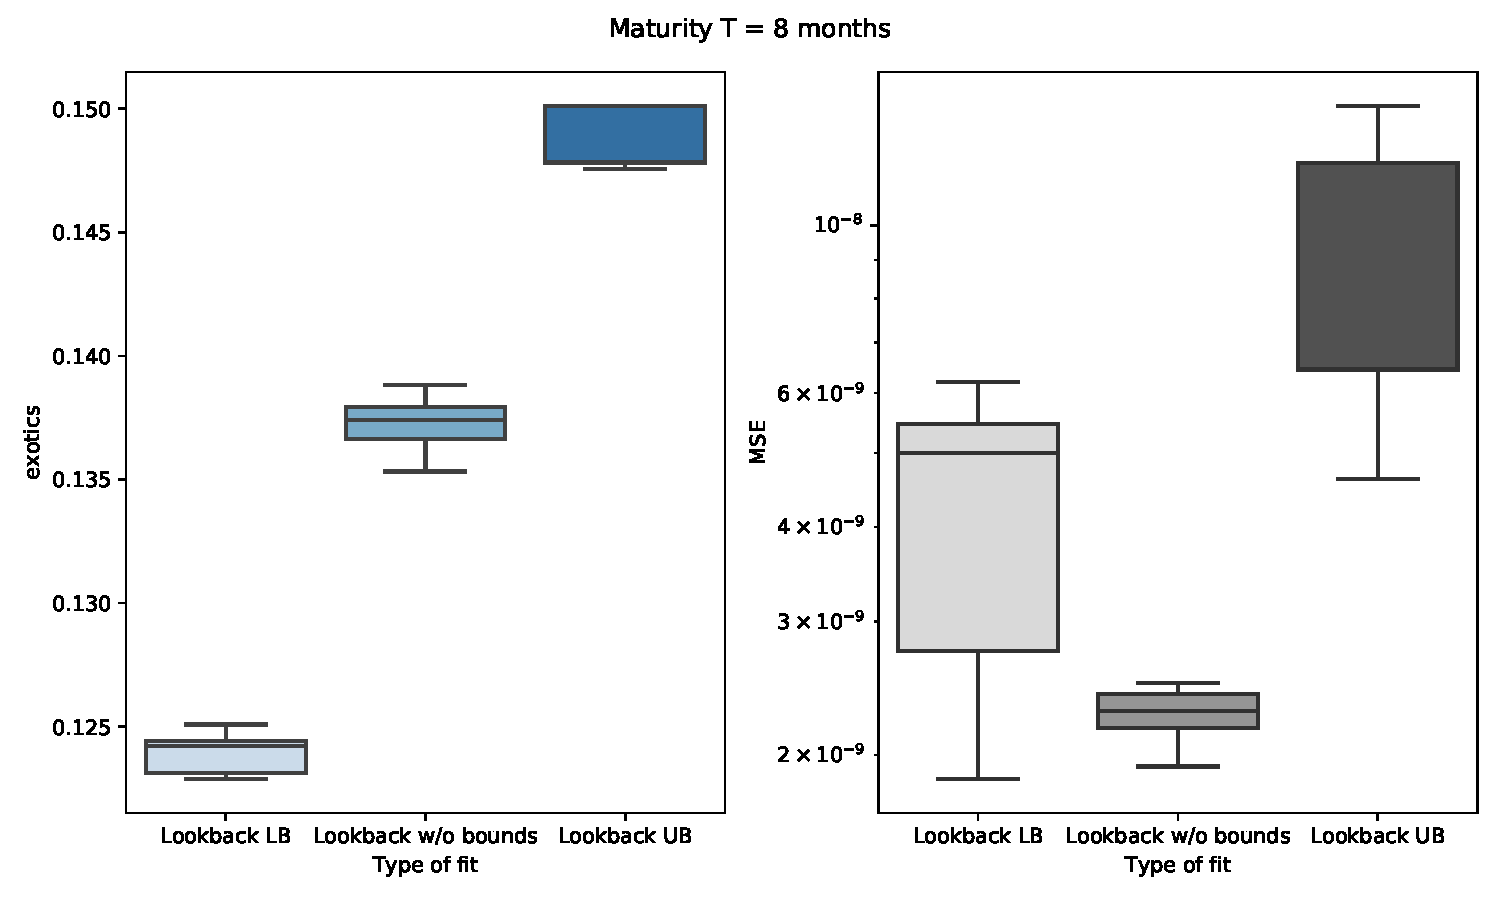
\includegraphics[width=0.45\textwidth]{content/reschap1/content/reschap1/Figures/figures_LV/BoxMaturity64}	
%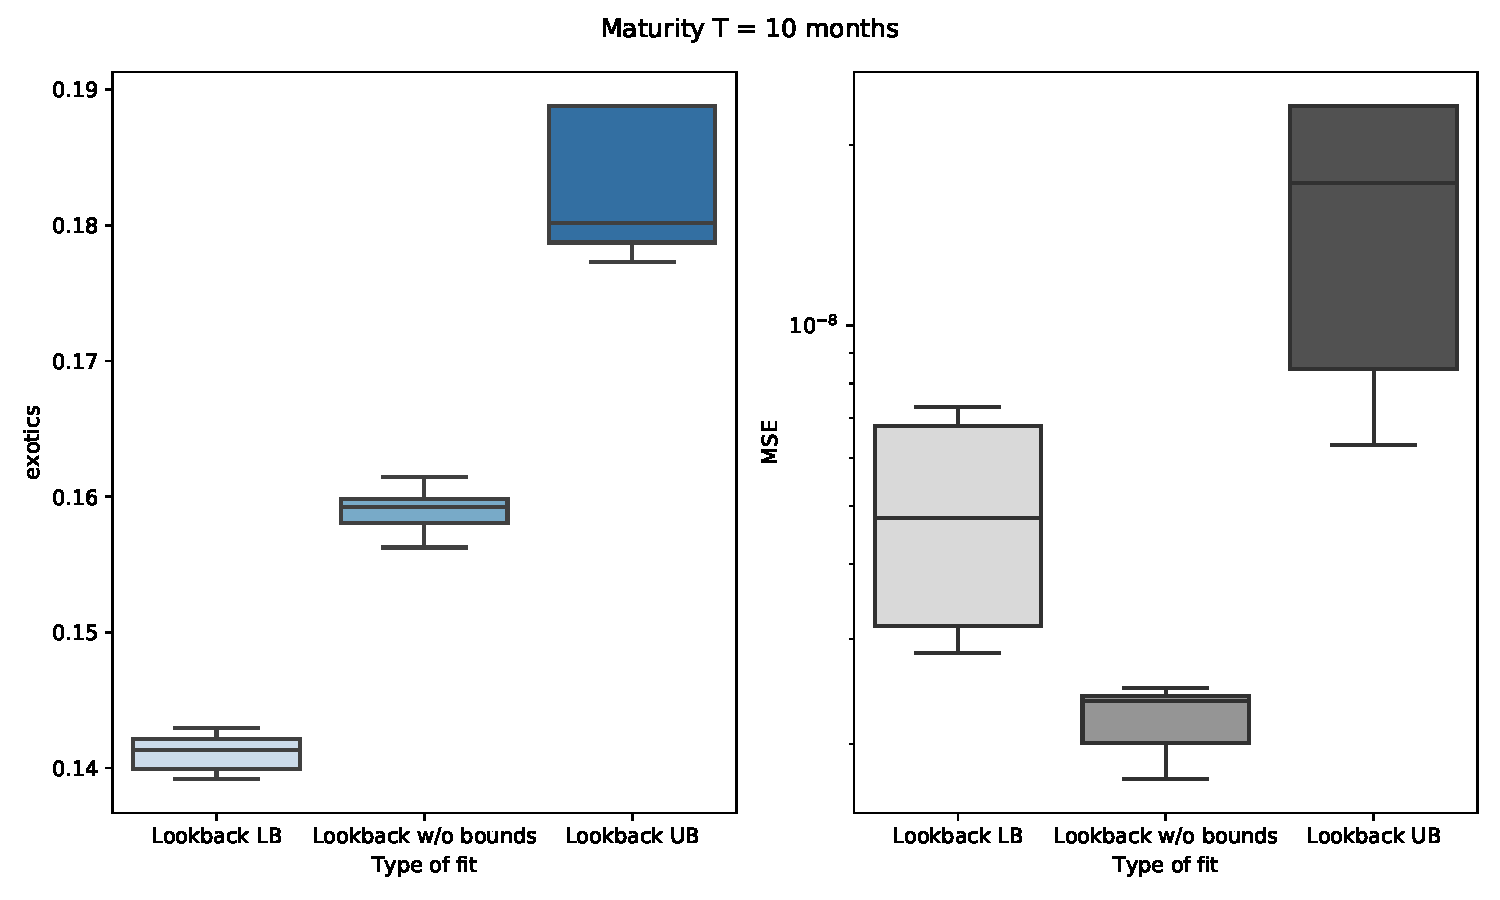
\includegraphics[width=0.45\textwidth]{content/reschap1/Figures/figures_LV/BoxMaturity80}
%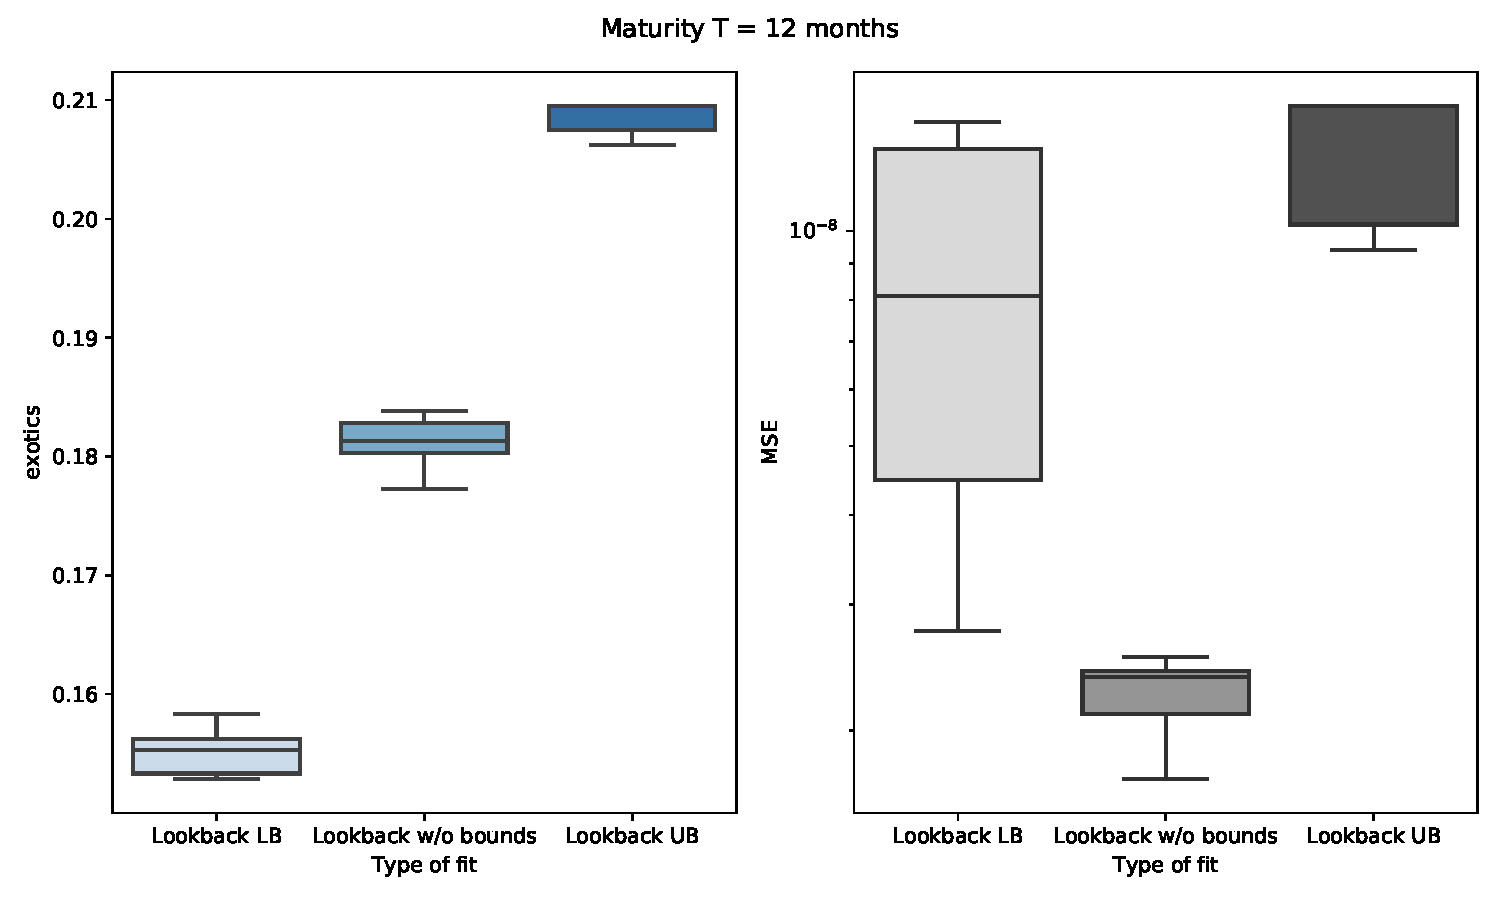
\includegraphics[width=0.45\textwidth]{content/reschap1/Figures/figures_LV/BoxMaturity96}
%\caption{Box plots for the Local Volatility model~\eqref{NeuralLV}. 
%Exotic option price quantiles are in blue in the left-hand box-plot groups.
%The MSE quantiles of market data calibration is in grey, in the right-hand box-plot groups. 
%Each box plot comes from 10 different runs of neural SDE calibration. 
%The three box-plots in each group arise respectively from aiming for a lower bound of the illiquid derivative (left), only calibrating to the market and then pricing the illiquid derivative (middle) and aiming for an upper bound of the illiquid derivative (right).}
%\label{fig LV boxplots}
%\end{figure}




%\subsection{Conclusions from calibrating for LV neural SDE}
%Each calibration is run~$10$ times with different initialisations of the network parameters, with the goal to check the robustness of the exotic option price 
%~$\EE^{\QQ(\theta)}[\Psi]$ for each calibrated neural SDE. 
%The blue boxplots in Figure~\ref{fig LV boxplots} provide different quantiles for the exotic option 
% price~$\EE^{\QQ(\theta)}[\Psi]$ and the obtained bounds after running. We make the following observations from calibrating LV neural SDE:
%\begin{enumerate}[i)]
%\item It is possible to obtain high accuracy of calibration with MSE of about~$10^{-9}$ for~$6$ month maturity, about~$10^{-8}$ for 12-month maturity when the only target is to fit market data. If we are minimizing / maximizing the illiquid derivative price at the same time, then the MSE increases somewhat so that it is about~$10^{-8}$ for both~$6$ and~$12$ month maturities. 
%See Figure~\ref{fig LV boxplots}. 
%The calibration has been performed using~$K=21$ strikes.
%\item The calibration is accurate not only in terms of MSE on prices but also individual implied volatility curves, see Figure~\ref{FigUnc}
% and others in Appendix~\ref{LVfitquality}.
%\item As we increase the number of strikes per maturity the range of possible values for the illiquid derivative narrows. 
%See Figure~\ref{Strikechart} and Tables~\ref{InitialisationImpact11strikes}, \ref{InitialisationImpact21strikes}, \ref{InitialisationImpact31strikes} and~\ref{InitialisationImpact41strikes}.
%One expects, assuming sufficient expressiveness of the neural network, that as the number of strikes (and maturities) would increase to infinity we would recover the unique~$\sigma$ given by the Dupire formula that fits the continuum of European option prices.
%\item With a limited amount of market data (which is closer to practical applications) even the LV neural SDE produces noticeable ranges for prices of illiquid derivatives, see again Figure~\ref{fig LV boxplots}.  
%\end{enumerate}
%
%
%\begin{figure}[h]
%\centering 
%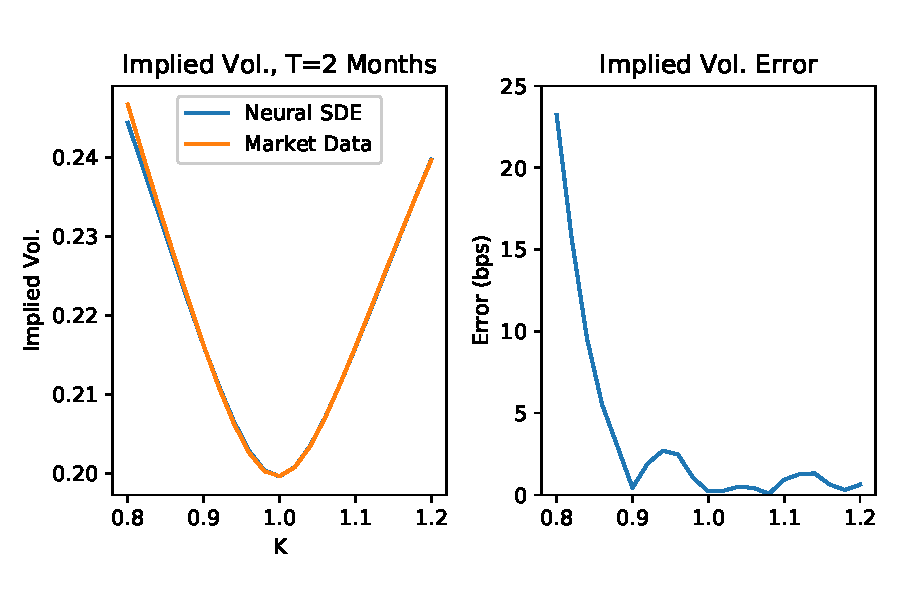
\includegraphics[clip,width=0.3\textwidth]{content/reschap1/Figures/figures_LV/Neural_SDE_maturity16_iv}
%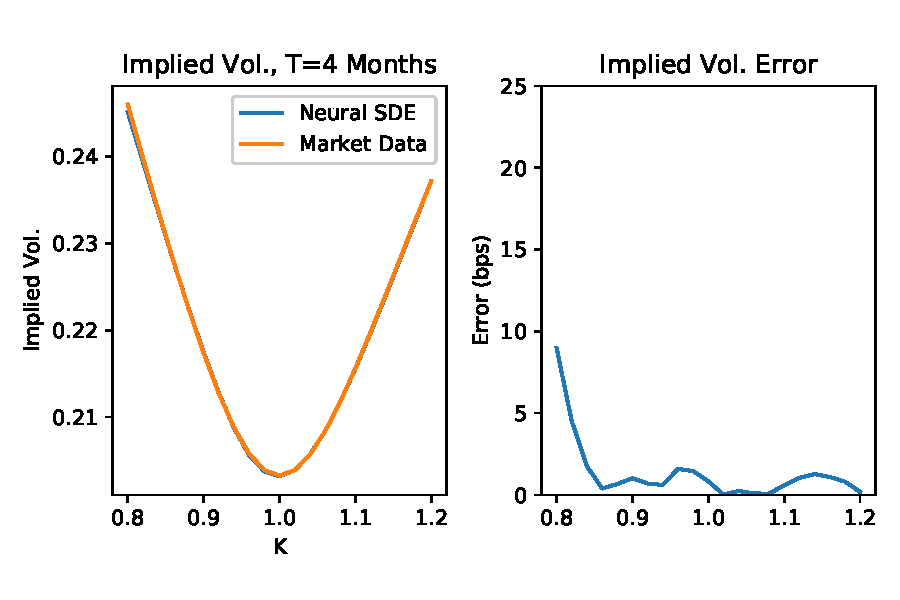
\includegraphics[clip,width=0.3\textwidth]{content/reschap1/Figures/figures_LV/Neural_SDE_maturity32_iv}
%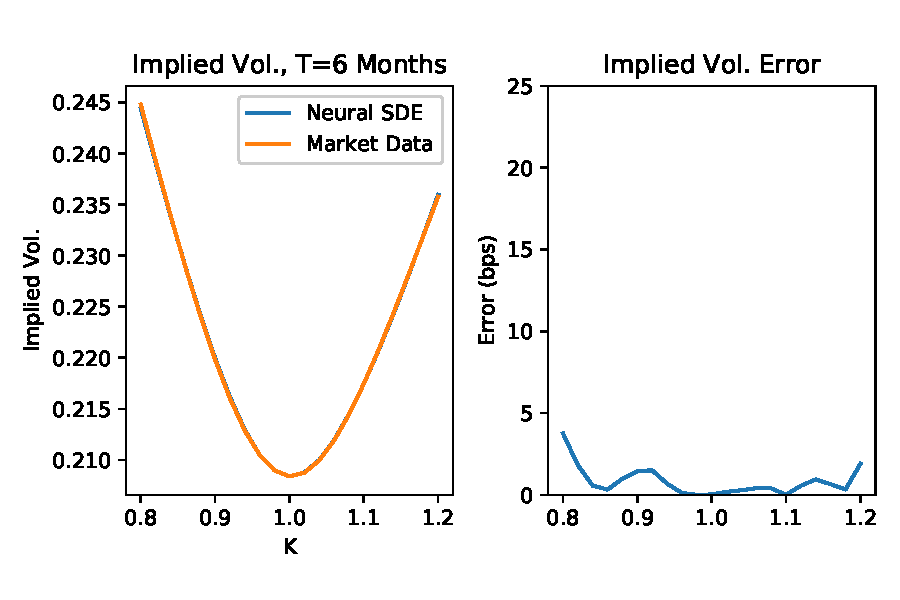
\includegraphics[clip,width=0.3\textwidth]{content/reschap1/Figures/figures_LV/Neural_SDE_maturity48_iv} 
%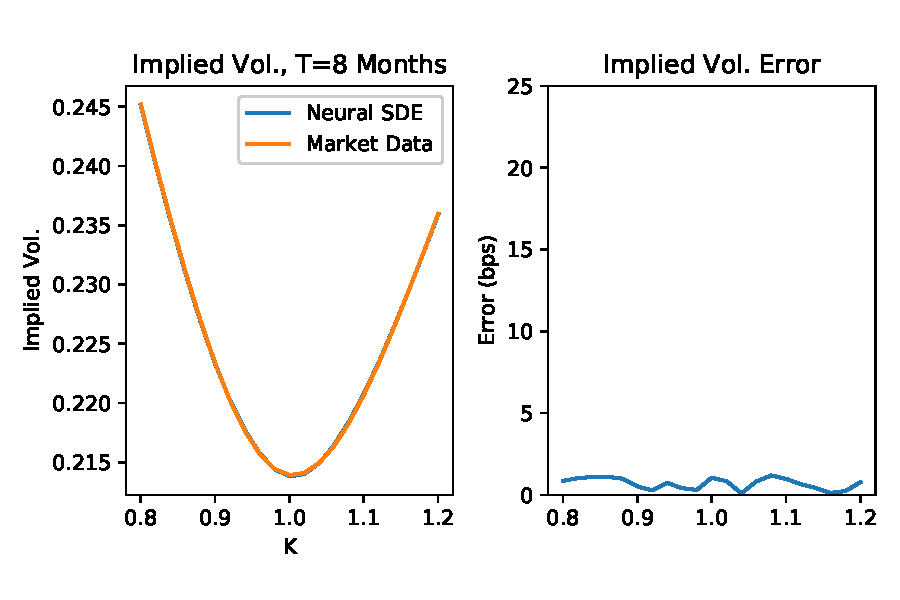
\includegraphics[clip,width=0.3\textwidth]{content/reschap1/Figures/figures_LV/Neural_SDE_maturity64_iv}
%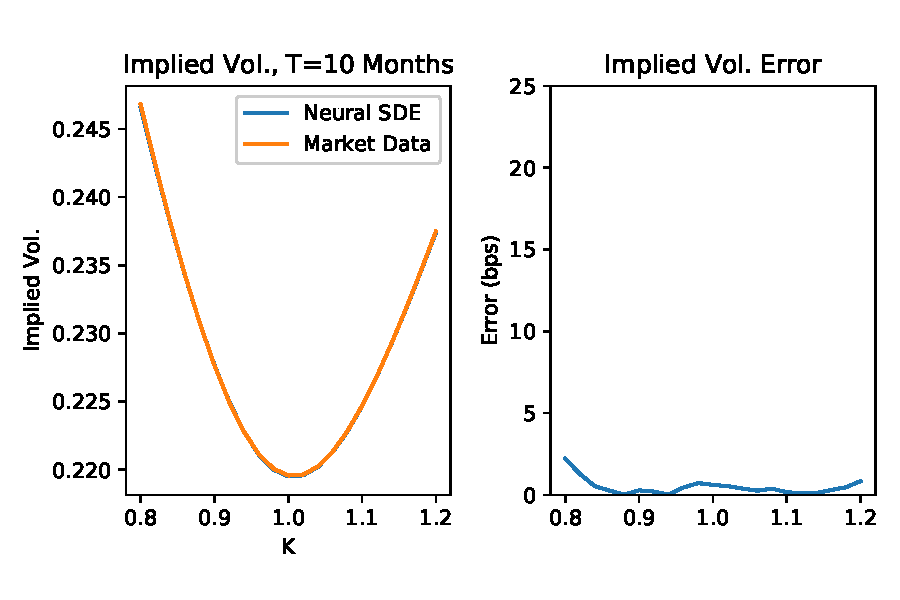
\includegraphics[clip,width=0.3\textwidth]{content/reschap1/Figures/figures_LV/Neural_SDE_maturity80_iv} 
%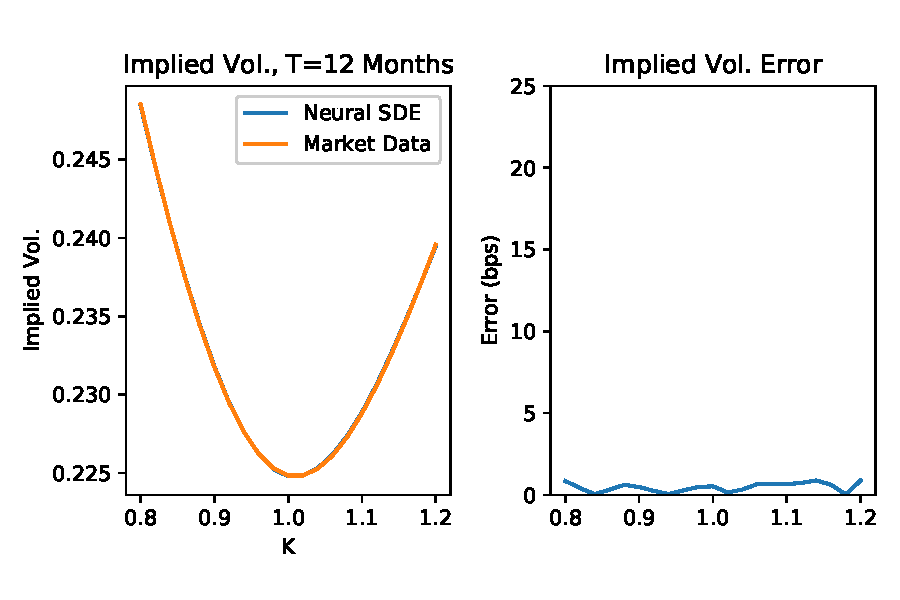
\includegraphics[clip,width=0.3\textwidth]{content/reschap1/Figures/figures_LV/Neural_SDE_maturity96_iv}
%\caption{Calibrated neural SDE LV model and target numbers implied volatility comparison.}
%\label{FigUnc}
%\end{figure}
%
%
%In Appendix~\ref{LVtables} we provide more details on how different random seeds, different constrained optimization algorithms and different number of strikes used in the market data input affect the illiquid derivative price.  
%
%In Appendix~\ref{LVfitquality} we present market price and implied volatility fit for constrained and unconstrained calibrations. 
%High level of accuracy in all calibrations is achieved due to the hedging neural network incorporated into model training.
%
%
%\begin{figure}[h]
%  \centering
%  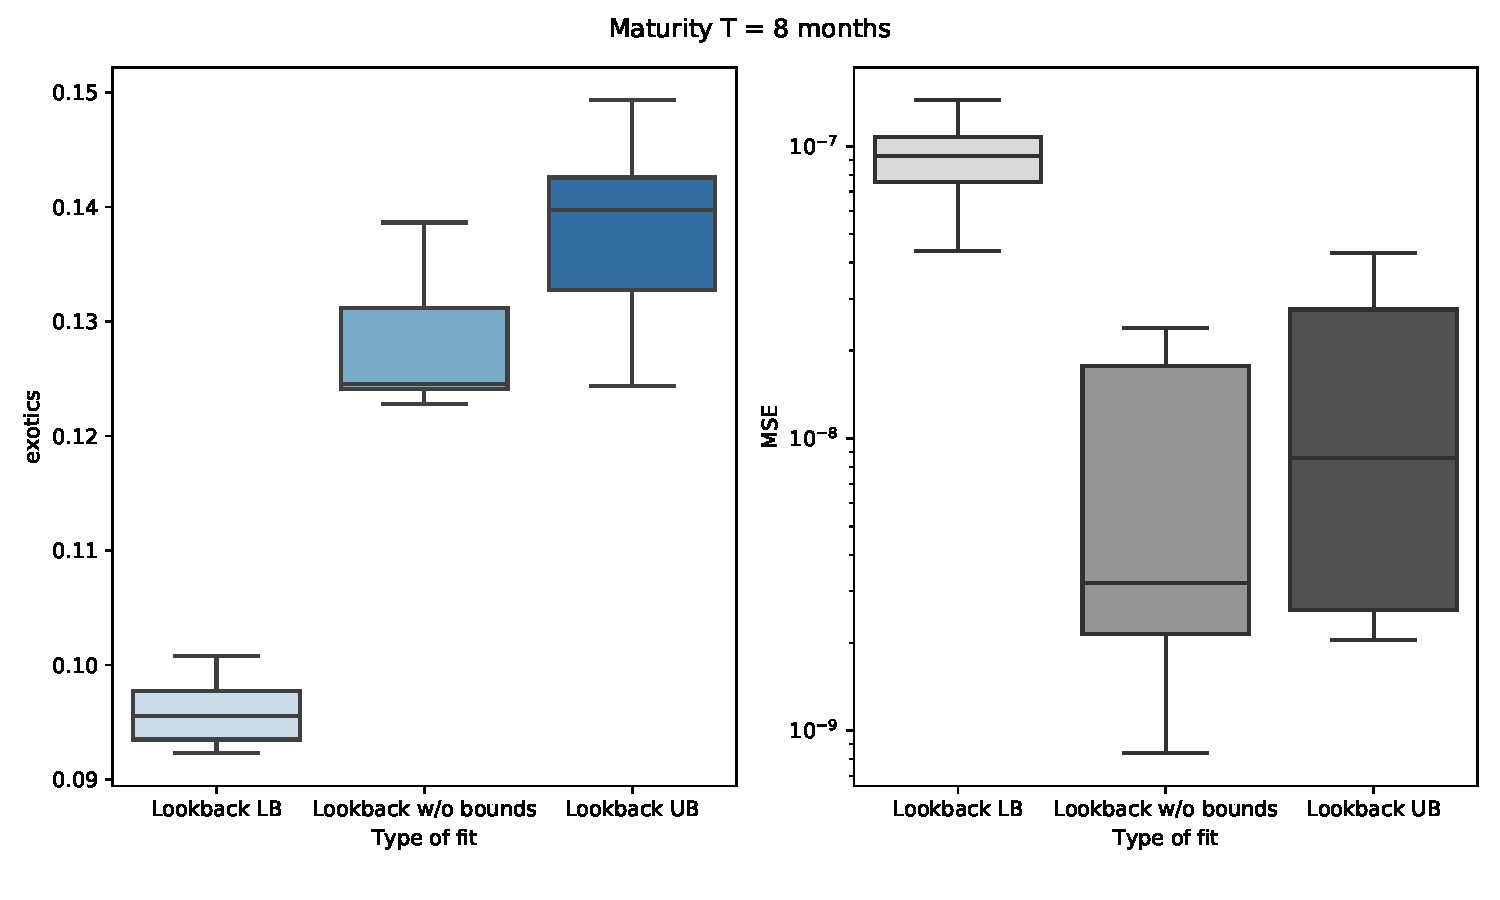
\includegraphics[clip,width=0.45\textwidth]{content/reschap1/Figures/figures_LSV/lookback_bound_augmented_lagrangian_maturity64}	
%  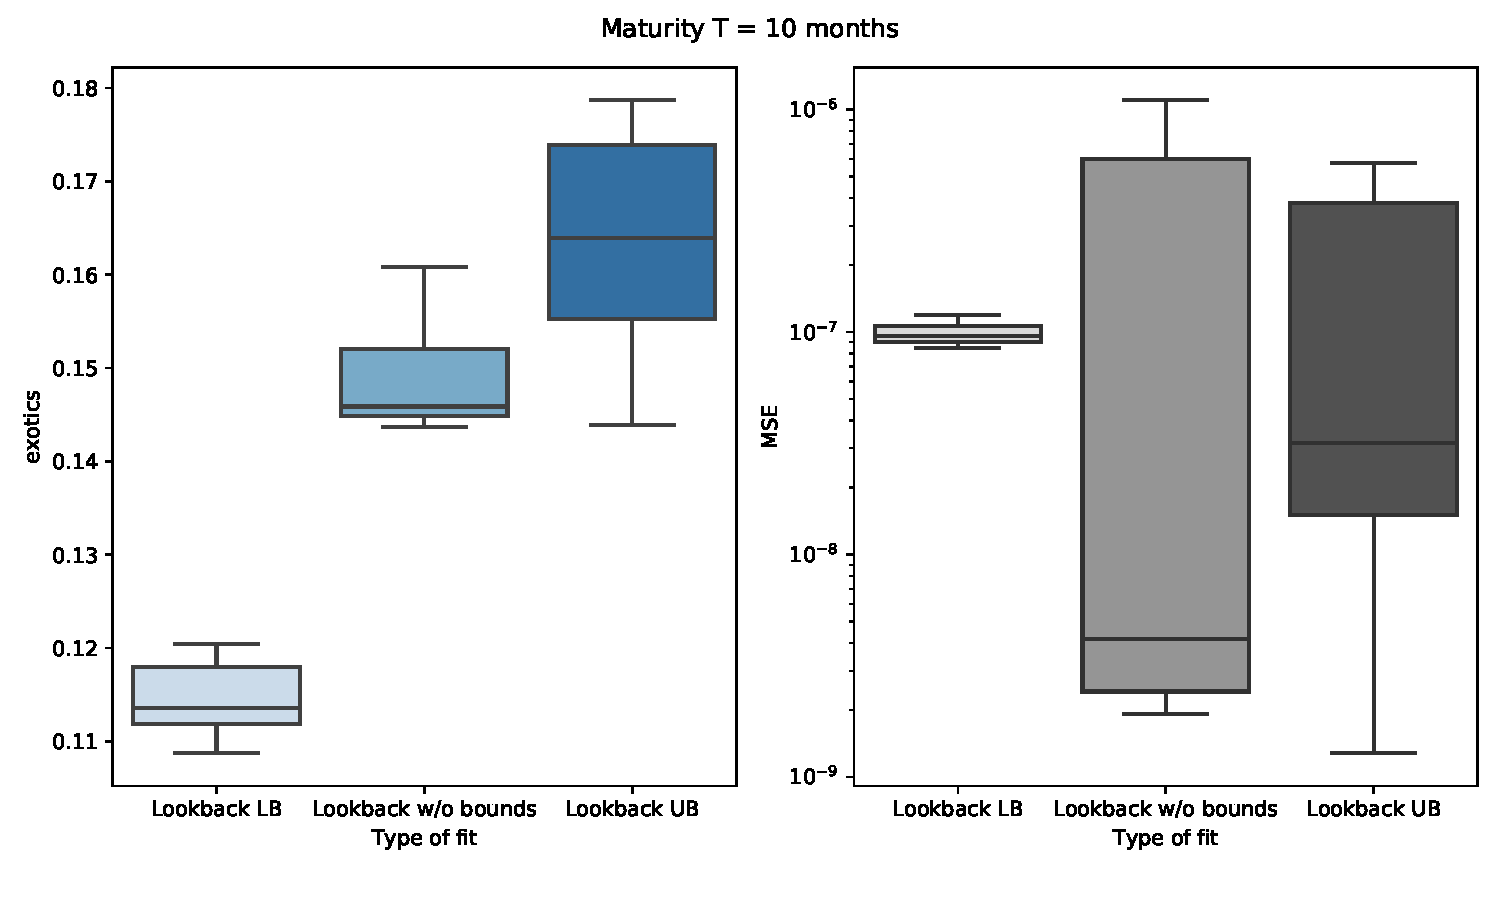
\includegraphics[clip,width=0.45\textwidth]{content/reschap1/Figures/figures_LSV/lookback_bound_augmented_lagrangian_maturity80}
%  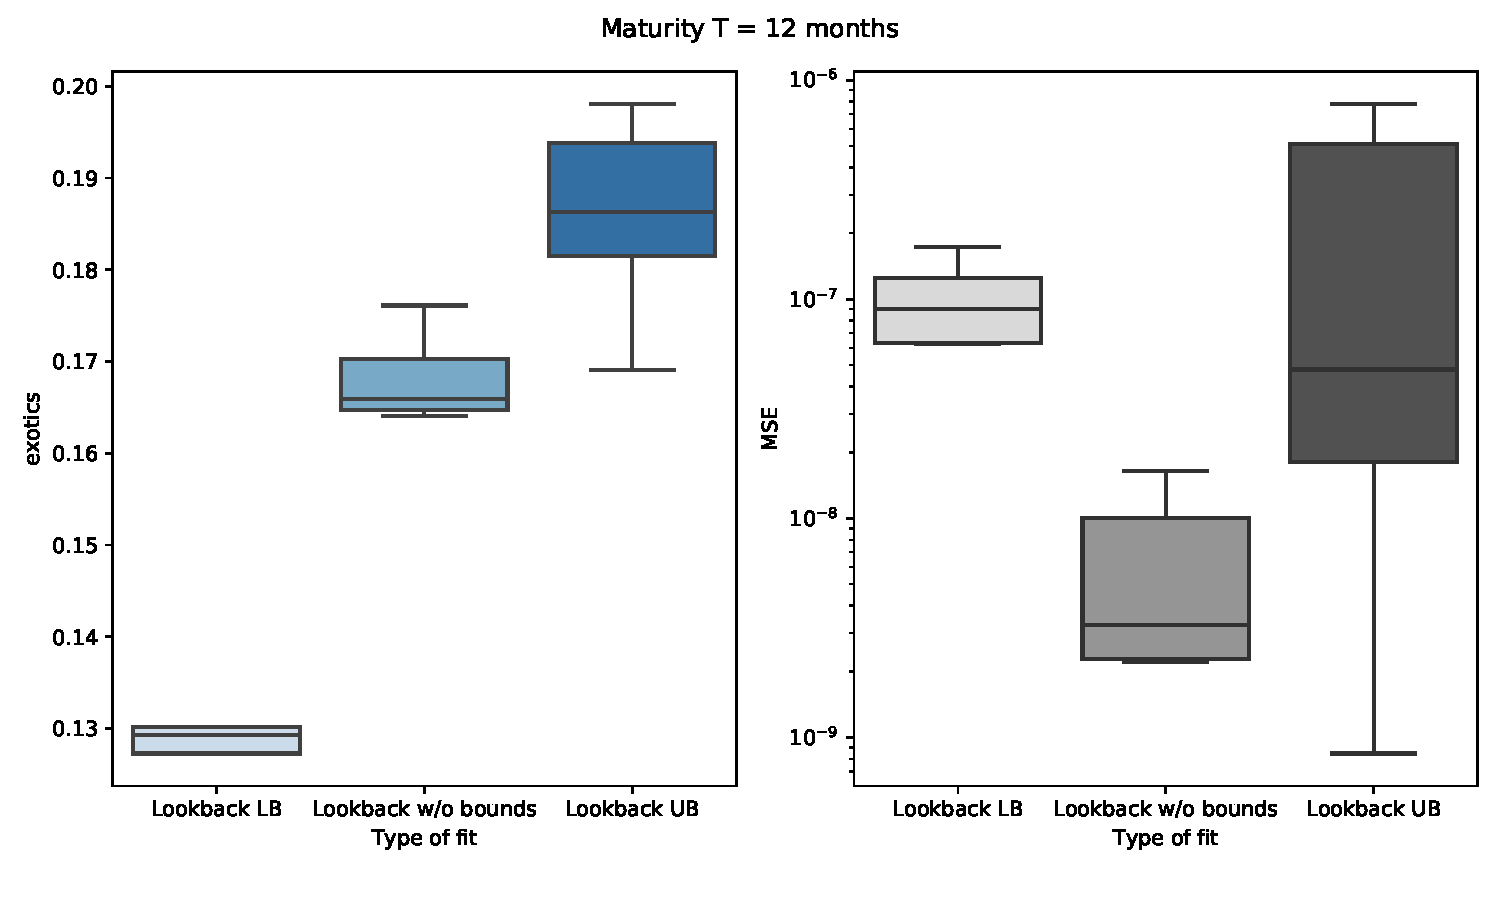
\includegraphics[clip,width=0.45\textwidth]{content/reschap1/Figures/figures_LSV/lookback_bound_augmented_lagrangian_maturity96} 
%  \caption{Box plots for the Local Stochastic Volatility model~\eqref{eq LSV SDE}. Exotic option price quantiles are in blue in the left-hand box-plot groups.
%The MSE quantiles of market data calibration is in grey, in the right-hand box-plot groups. 
%Each box plot comes from 10 different runs of neural SDE calibration. 
%The three box-plots in each group arise respectively from aiming for a lower anound of the illiquid derivative(left), only calibrating to market and then pricing the illiquid derivative (middle) and aiming for a upper bound of the illiquid derivative (right).}
%\label{fig LSV boxplots}
%\end{figure}
%
%
%
%\subsection{Conclusions from calibrating for LSV neural SDE}
%Each calibration is run ten times with different initialisations of the network parameters, with the goal to check the robustness of the exotic option price 
%~$\EE^{\QQ(\theta)}[\Psi]$ for each calibrated neural SDE. 
%The blue boxplots in Figure~\ref{fig LSV boxplots} provide different quantiles for the exotic option 
% price~$\EE^{\QQ(\theta)}[\Psi]$ and the obtained bounds after running all the experiments~$10$ times. 
%We make the following observations from calibrating LSV neural SDE:
%\begin{enumerate}[i)]
%\item We note that our methods achieve high calibration accuracy to the market data (measured by MSE) with consistent bounds on the exotic option prices. 
%See Figure~\ref{fig LSV boxplots}.
%\item The calibration is accurate not only in MSE on prices but also individual implied volatility curves, see Figure~\ref{fig LSV calibration}
% and others in Appendix~\ref{sec LSVfitquality}.
%\item The LSV neural SDE produces noticeable ranges for prices of illiquid derivatives, see again Figure~\ref{fig LSV boxplots}.  
%\end{enumerate}
%
%
%\begin{figure}[h]
%  \centering 
%  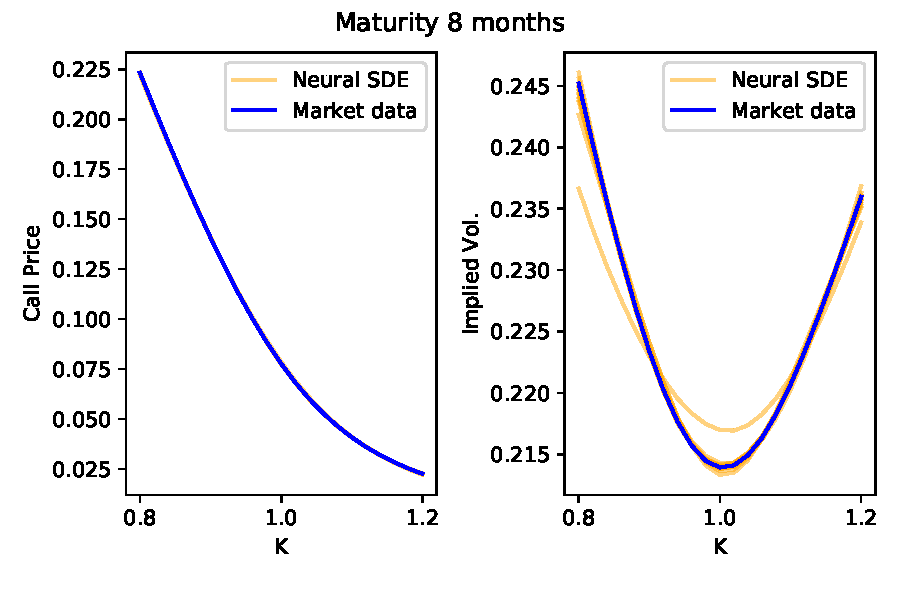
\includegraphics[clip,width=0.3\textwidth]{content/reschap1/Figures/figures_LSV/maturity_64}
%  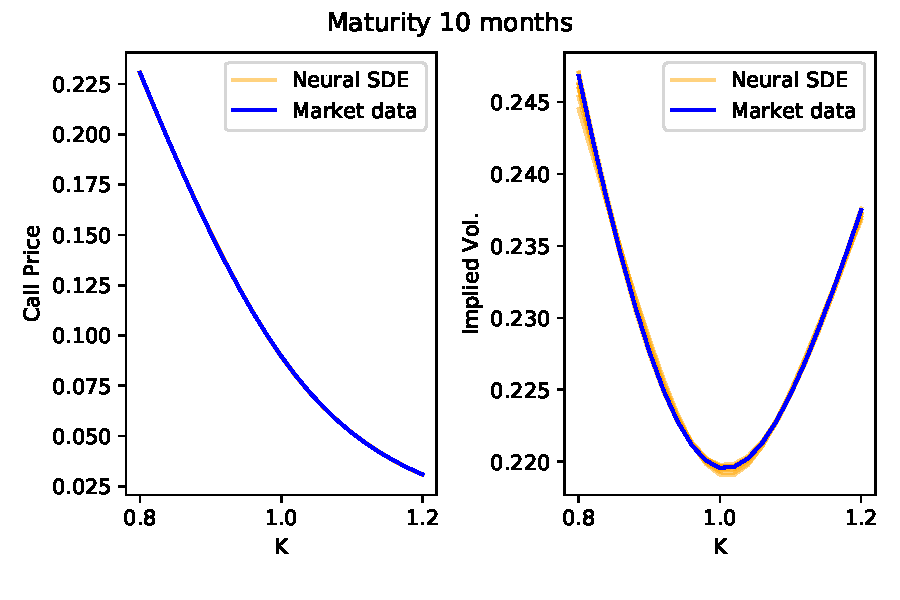
\includegraphics[clip,width=0.3\textwidth]{content/reschap1/Figures/figures_LSV/maturity_80}
%  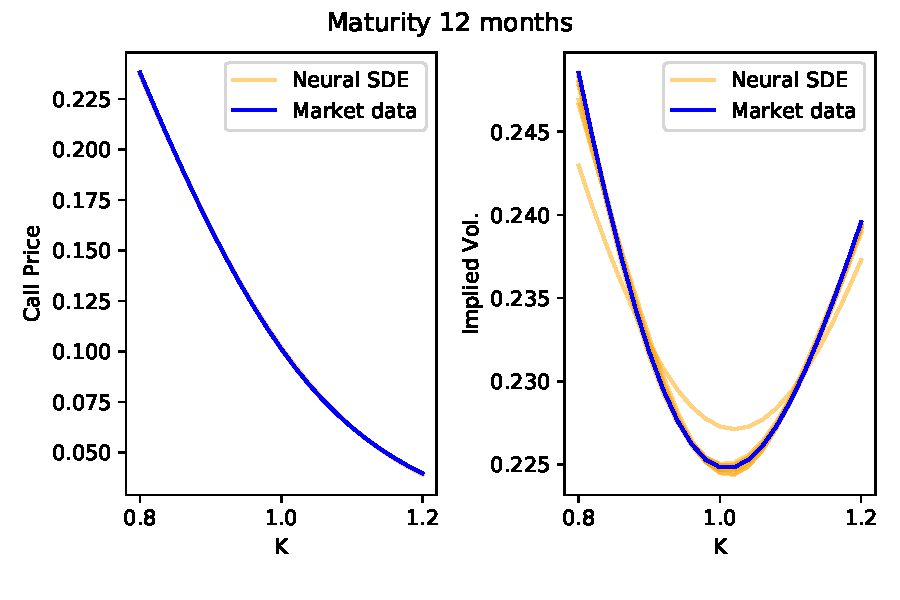
\includegraphics[clip,width=0.3\textwidth]{content/reschap1/Figures/figures_LSV/maturity_96} 
%  \caption{Comparing market and model data fit for the neural SDE LSV model~\eqref{eq LSV SDE} when targeting only the {\em market data}.
%We see vanilla option prices and implied volatility curves of the 10 calibrated neural SDEs vs. the market data for different maturities.
%}
%\label{fig LSV calibration}  
%\end{figure}


%\subsection{Hedging strategy evaluation} We calculate the error of the portfolio hedging strategy of the lookback option 
%at maturity~$T=6$ months, given by the empirical variance for a trained set of parameters~$\tilde{\theta}\in\Theta\,$:
%\[
%\mathbb{V}\mathrm{ar}^{\QQ^N} \left[ \Psi\left(X^{\pi,\tilde{\theta}}\right)-\sum_{k=0}^{N_{\text{steps}}-1} \bar{\Hf}(t_k, (X_{t_k\wedge t_j}^{\pi,\tilde{\theta}})_{j=0}^{N_{\text{steps}}}, \xi_{\Psi})\Delta \bar S^{\pi,\tilde{\theta}}_{t_{k}} \right] \,.
%\]
%The histogram in Figure~\ref{fig hedge error} is calculated on~$N=400\, 000$ different paths and provides the values of~$s$,
%\[
%s\defEqual\Psi\left(X^{\pi,\tilde{\theta}}\right)-\sum_{k=0}^{N_{\text{steps}}-1} \bar{\Hf}(t_k, (X_{t_k\wedge t_j}^{\pi,\tilde{\theta}})_{j=0}^{N_{\text{steps}}}, \xi_{\Psi})\Delta \bar S^{\pi,\tilde{\theta}}_{t_{k}} - \EE^{\QQ^N}\left[\Psi\left(X^{\pi,\tilde{\theta}}\right)\right],
%\]
%i.e., such that 
%\[
%\EE^{\QQ^N}[s^2] = \mathbb{V}\mathrm{ar}^{\QQ^N} \left[ \Psi\left(X^{\pi,\tilde{\theta}}\right)-\sum_{k=0}^{N_{\text{steps}}-1} \bar{\Hf}(t_k, (X_{t_k\wedge t_j}^{\pi,\tilde{\theta}})_{j=0}^{N_{\text{steps}}}, \xi_{\Psi})\Delta \bar S^{\pi,\tilde{\theta}}_{t_{k}} \right]. 
%\]
%We obtain~$\EE^{\QQ^N}[s^2] = 1.6\times 10^{-3}$.
%%\begin{equation}\label{eq loss cv real}
%%\bar \xi^{\ast} \in  \argmin_{\bar \xi} \mathbb V\text{ar}\left[\phi((X_t)_{t\in[0,T]}) -  \int_0^T \bar {\Hf}(r,(X_{r\wedge t})_{t\in[0,T]},\bar \xi) \,d \bar S^\theta_r \bigg | \Ff_0\right]
%%\end{equation}
%%
%%
%%\[
%%\mathcal E = \Phi - \EE[\Phi | \mathcal F_0] - \int_0^T Z_s \, \D W_s\
%%\]
%
%\begin{figure}[h]\label{fig hedge error}
%\centering
%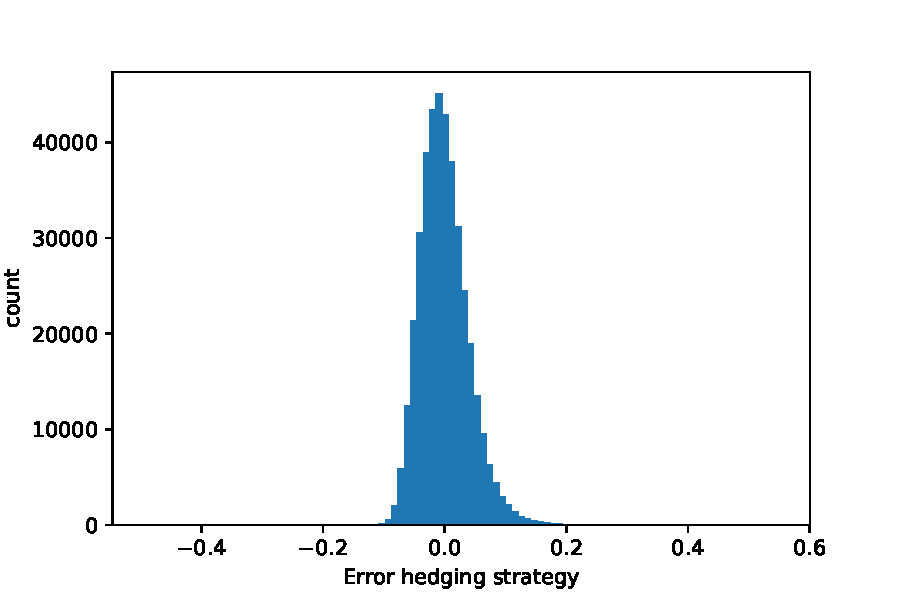
\includegraphics[clip,width=0.6\textwidth]{content/reschap1/Figures/figures_LSV/hedging_error}
%\caption{Error of the portfolio hedging strategy for the lookback option}	
%\end{figure}
%



%Finally, we study the effect of the control variate parametrisation on the learning speed
%in Algorithm~\ref{alg LSV calibration vanilla}.
%Figure~\ref{fig test cv} displays the evolution of the Root Mean Squared Error of two runs of 
%calibration to market vanilla option prices for two-months maturity: the blue line using Algorithm~\ref{alg LSV calibration vanilla} with simultaneous learning of the hedging strategy, and the orange line without the hedging 
%strategy. 
%We recall that from Section~\ref{sec many maturities}, the Monte Carlo estimator~$\partial_{\theta}h^{N}(\theta)$ is a biased estimator of 
%$\partial_{\theta}h(\theta)$
%An upper bound of the bias is given by Corollary~\ref{eq cor sq loss bias}, that shows
%that by reducing the variance of the Monte Carlo estimator of the option price then the bias of~$\partial_{\theta}h^{N}(\theta)$ is also reduced, yielding better convergence behaviour of the 
%stochastic approximation algorithm. 
%This can be observed in Figure~\ref{fig test cv}. 
%\begin{figure}[h]
%  \centering 
%  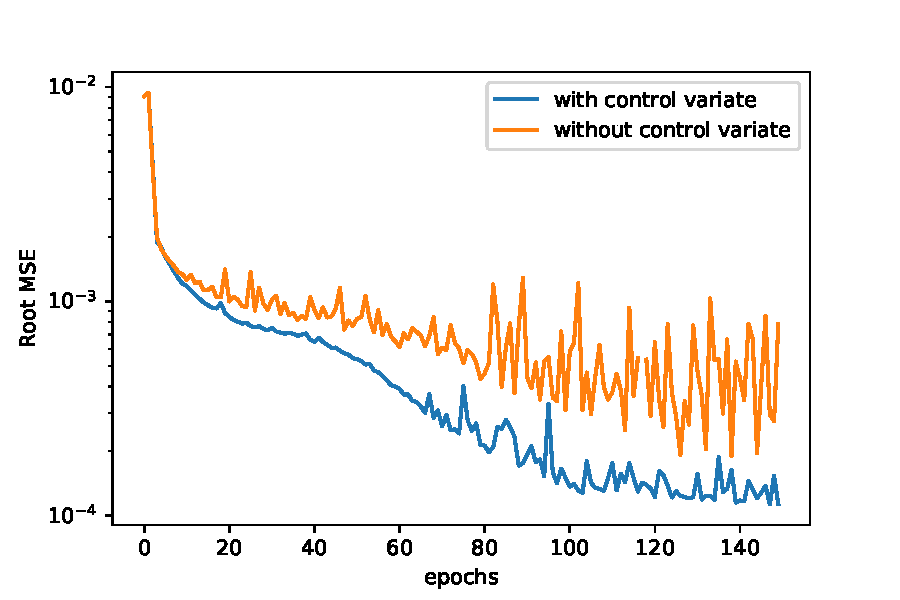
\includegraphics[clip,width=0.6\textwidth]{content/reschap1/Figures/figures_LSV/test_calibration_cv}
%  \caption{Root Mean Squared Error of calibration to Vanilla option prices with and without hedging strategy parametrisation}
%  \label{fig test cv}
%\end{figure}


%\section{Data used in calibration to real data} \label{sec:real data}
%%\begin{table}[H]
%%\caption{SPX call prices. Maturities~$T$ are measured in months. For training purposes, data is scaled by a factor of~$10^{-3}$. }
%%\label{table:data}
%%\centering
%\begin{tabularx}{\textwidth}{|l||X|X|X|X|X|X|X|}
%\toprule
%Strike & T = 1 & T = 2 & T = 3 & T = 4 & T = 5 & T = 6   \\
%\midrule \midrule
%K = 2825  & 402.0 & 406.9 & 413.15 & 421.25 & 428.1 & 437.6 \\  \midrule
%K = 2850  & 377.0 & 383.0 & 389.85 & 398.45 & 406.0 & 415.85 \\  \midrule
%K = 2875  & 352.3 & 359.1 & 366.7 & 375.85 & 383.95 & 394.2 \\  \midrule
%K = 2900  & 327.7 & 335.35 & 343.65 & 353.45 & 361.75 & 372.8 \\  \midrule
%K = 2925  & 303.45 & 311.7 & 320.8 & 330.95 & 340.3 & 351.4 \\  \midrule
%K = 2950  & 279.0 & 288.3 & 298.2 & 309.05 & 318.65 & 330.75 \\  \midrule
%K = 2975  & 254.65 & 265.0 & 275.95 & 287.5 & 297.65 & 309.9 \\  \midrule
%K = 3000  & 230.3 & 242.0 & 253.9 & 266.0 & 276.7 & 289.5 \\  \midrule
%K = 3025  & 206.3 & 219.15 & 232.1 & 244.65 & 256.65 & 269.4 \\  \midrule
%K = 3050  & 182.45 & 196.95 & 210.8 & 224.45 & 236.4 & 249.7 \\  \midrule
%K = 3075  & 158.8 & 174.7 & 189.75 & 204.0 & 216.45 & 230.2 \\  \midrule
%K = 3100  & 135.5 & 153.15 & 169.25 & 184.0 & 196.9 & 211.1 \\  \midrule
%K = 3125  & 112.4 & 132.35 & 149.35 & 164.55 & 177.85 & 192.4 \\  \midrule
%K = 3150  & 90.3 & 111.95 & 130.05 & 145.55 & 159.25 & 174.2 \\  \midrule
%K = 3175  & 69.25 & 92.45 & 111.5 & 127.3 & 141.05 & 156.65 \\  \midrule
%K = 3200  & 49.55 & 74.2 & 93.95 & 109.9 & 123.8 & 139.6 \\  \midrule
%K = 3225  & 32.5 & 57.5 & 77.55 & 93.5 & 107.4 & 123.3 \\  \midrule
%K = 3250  & 19.3 & 42.95 & 62.65 & 78.25 & 92.05 & 107.8 \\  \midrule
%K = 3275  & 10.2 & 30.85 & 49.4 & 64.35 & 77.8 & 93.3 \\  \midrule
%K = 3300  & 5.05 & 21.4 & 38.15 & 51.95 & 64.8 & 79.85 \\  \midrule
%K = 3325  & 2.35 & 14.45 & 28.75 & 41.25 & 53.3 & 67.6 \\  \midrule
%K = 3350  & 1.15 & 9.6 & 21.3 & 32.2 & 43.2 & 56.6 \\  \midrule
%K = 3375  & 0.62 & 6.45 & 15.7 & 24.85 & 34.5 & 46.75 \\  \midrule
%K = 3400  & 0.35 & 4.35 & 11.5 & 19.0 & 27.35 & 38.25 \\  \midrule
%K = 3425  & 0.28 & 2.98 & 8.4 & 14.5 & 21.5 & 31.0 \\  \midrule
%K = 3450  & 0.22 & 2.05 & 6.25 & 11.05 & 16.9 & 25.05 \\  \midrule
%K = 3475  & 0.18 & 1.45 & 4.65 & 8.45 & 13.3 & 20.1 \\  \midrule
%K = 3500  & 0.15 & 1.02 & 3.55 & 6.55 & 10.5 & 16.25 \\  \midrule
%K = 3525  & 0.15 & 0.77 & 2.65 & 5.1 & 8.35 & 13.1 \\  \midrule
%K = 3550  & 0.1 & 0.57 & 2.05 & 4.0 & 6.7 & 10.7 \\  \midrule
%K = 3575  & 0.08 & 0.45 & 1.55 & 3.15 & 5.4 & 8.75 \\  \midrule
%K = 3600  & 0.08 & 0.35 & 1.2 & 2.5 & 4.35 & 7.1 \\  \midrule
%K = 3650  & 0.08 & 0.25 & 0.75 & 1.6 & 2.9 & 4.85 \\  \midrule
%\bottomrule
%\caption{SPX call prices. Maturities~$T$ are measured in months. For training purposes, data is scaled by a factor of~$10^{-3}$. }
%\end{tabularx}
%%\end{table}	


%\section{Data used in calibration to synthetic data}\label{CalData}
%
%We used the Heston model to generate prices of calls and puts. The model is
%\begin{eqnarray}\label{CalDataEq}
%dX_t &=& r X_t\D t + X_t \sqrt{V_t}\D W_t, \quad X_0 = x_0 \\
%dV_t &=& \kappa (\mu - V_t)dt + \eta \sqrt{V_t}dB_t, \quad V_0 = v_0 \\
%d\langle B, W \rangle_t &=& \rho\D t\,.
%\end{eqnarray}
%It is well known that for this model a semi-analytic formula can be used to calculate option prices, see~\cite{heston1997closed} but also~\cite{LHT}. 
%The parameters below were used to generate target model calibration prices and were chosen so that the model produces a large skew at the short end of the smile:
%\begin{equation}
%\label{eq heston params}
%x_0 = 1,~ r = 0.025\,, \,\,\, \kappa= 0.78\,, \,\,\, \mu = 0.11\,, \,\,\, \eta =0.68\,, \,\,\, V_0 =0.04\,, \,\,\, \rho = 0.044,
%\end{equation}
%
%\begin{figure}[h!tbp]
%  \centering 
%  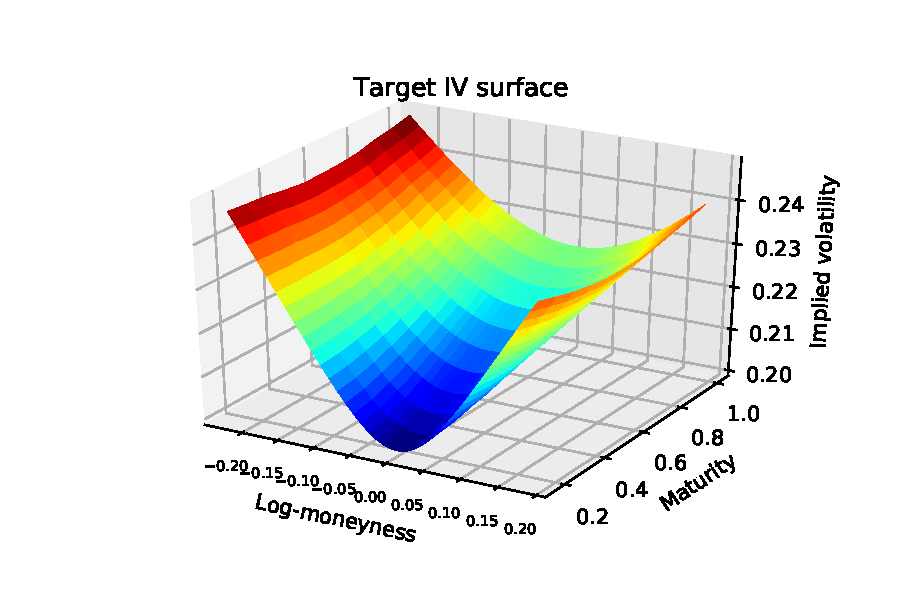
\includegraphics[width=0.45\textwidth]{content/reschap1/Figures/figures_LV/IV_more_points}
%\caption{The ``market'' data used in the calibration of the neural SDE models. 
%In fact the implied volatility surface comes from~\eqref{CalDataEq} and~\eqref{eq heston params}.}
%\label{TargetIVs}
%\end{figure}
%
%
%Options with bi-monthly maturities of up to one year with varying ranges of strikes were used as market data for neural SDE calibration.
%The call / put option prices were obtained from the Heston model using Monte Carlo simulation with~$10^7$ Brownian trajectories.
%We use bi-monthly maturities of up to one year for considered calibrations. A varying range of strikes is used among different calibrations. 
%%See Figure~\ref{TargetIVs} for the resulting ``market'' data.




%\section{Feed-forward neural networks}
%\label{FFNNs}
%
%
%
%Feed-forward neural networks are functions constructed by the composition of affine map and non-linear activation function.
%We fix a locally Lipschitz activation function~$\mathbf a:\RR \to \RR$ as \texttt{relu}  function~$a(z)=\max(0,z)$ and
%for~$d\in \NN$ define~$\mathbf A_d : \RR^d \to \RR^d$ as the function given, for~$x=(x_1,\ldots,x_d)$ by 
%$\mathbf A_d(x) = (\mathbf a(x_1),\ldots, \mathbf a(x_d))$.
%We fix~$L\in \NN$ (the number of layers),~$l_k \in \NN$,~$k=0,1,\ldots L-1$ (the size of input to layer~$k$) and~$l_L \in \NN$ (the size of the network output). 
%A fully connected artificial neural network is then given by~$\theta = ((W_1,B_1), \ldots, (W_L, B_L))$,
%where, for~$k=1,\ldots,L$, we have real~$l_{k-1}\times l_k$ matrices~$W_k$ and real~$l_k$ dimensional
%vectors~$B_k$. 	
%%Neural network parameters~$W_{k}$ and bias terms~$B_k$ are sampled from uniform distribution~$U[-\lambda,\lambda]$ with~$\lambda=\frac{1}{\sqrt{l_{k-1}}}$. 
%%We use ADAM optimiser with multistep learning rate scheduler and RMSE loss function. 
%
%The artificial neural network defines a function~$\mathcal R(\cdot, \theta) : \RR^{l_0} \to \RR^{l_L}$ given recursively, for~$x_0 \in \RR^{l_0}$, by 
%\[
%\mathcal R(x_0, \theta) = W_L x_{L-1} + B_L\,, \,\,\,\, 
%x_k = \mathbf A_{l_k}(W_k x_{k-1} + B_k)\,,k=1,\ldots, L-1\,.
%\]
%%We can also define the function~$\mathcal P$ which counts the number of parameters as 
%%\[
%%\mathcal P(\Phi) = \sum_{i=1}^L (l_{k-1}l_k + l_k )\,.
%%\]
%We will call such a class of fully connected artificial neural networks~$\mathcal{DN}$.
%Note that since the activation functions and architecture are fixed the learning task entails
%finding the optimal~$\theta \in \RR^{\mathcal P}$ where~$p$ is the number of parameters in
%$\theta$ given by
%\[
%\mathcal P(\theta) = \sum_{i=1}^L (l_{k-1}l_k + l_k )\,.
%\]
%


%\section{LV neural SDEs calibration accuracy}
%\label{LVfitquality}
%
%Figures~\ref{FigUnc}, \ref{FigLB}, \ref{FigUB} present implied volatility fit of the local volatility neural SDE model~\eqref{NeuralLV} calibrated to market vanilla data only; market vanilla data with a lower bound constraint on lookback option payoff; market vanilla data with an upper bound constraint on lookback option payoff respectively. 
%Figures~\ref{FigUncprice}, \ref{FigLBprice}, \ref{FigUBprice} present target option price fit of local volatility neural SDE model~\eqref{NeuralLV} calibrated to market vanilla data only; market vanilla data with a lower bound constraint on lookback option payoff; market vanilla data with an upper bound constraint on lookback option payoff respectively. 
%High level of accuracy in all calibrations is achieved due to the hedging neural network incorporated into model training.
%
%
%\begin{figure}[h]
%\centering 
%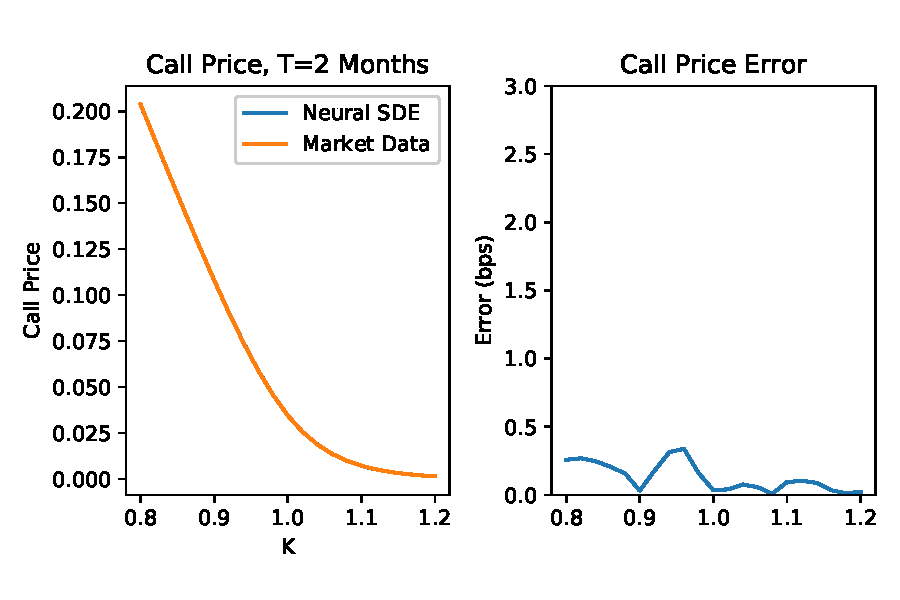
\includegraphics[clip,width=0.3\textwidth]{content/reschap1/Figures/figures_LV/Neural_SDE_maturity16_vanilla}
%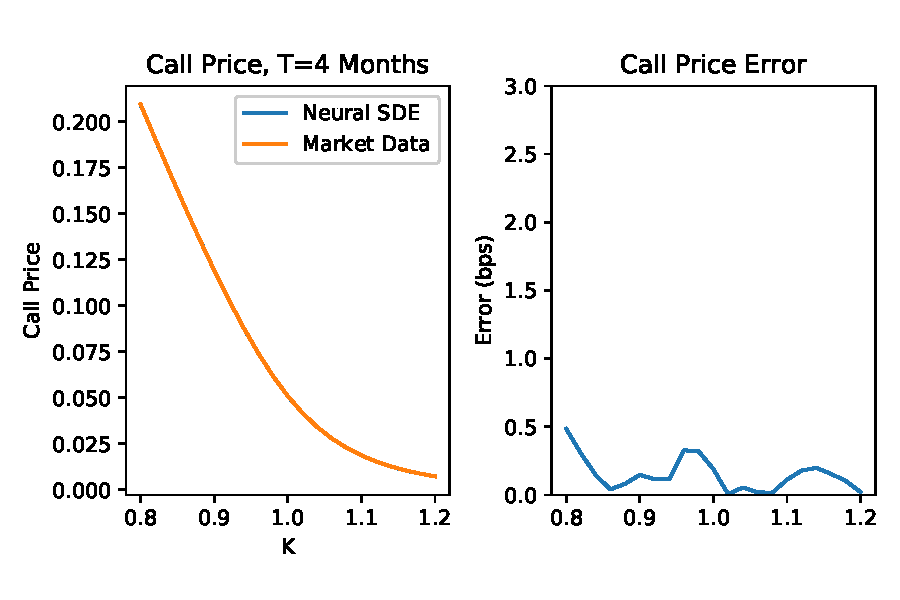
\includegraphics[clip,width=0.3\textwidth]{content/reschap1/Figures/figures_LV/Neural_SDE_maturity32_vanilla}
%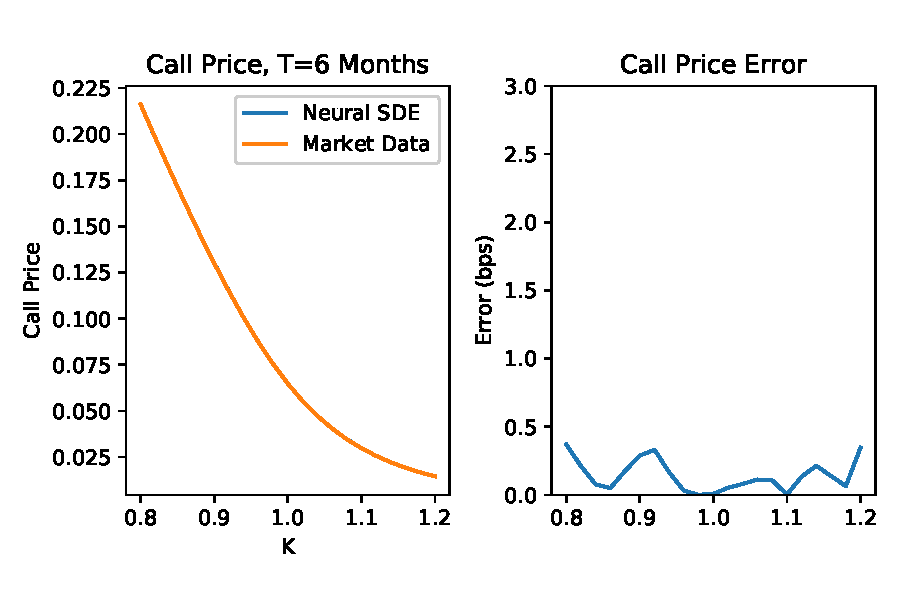
\includegraphics[clip,width=0.3\textwidth]{content/reschap1/Figures/figures_LV/Neural_SDE_maturity48_vanilla} 
%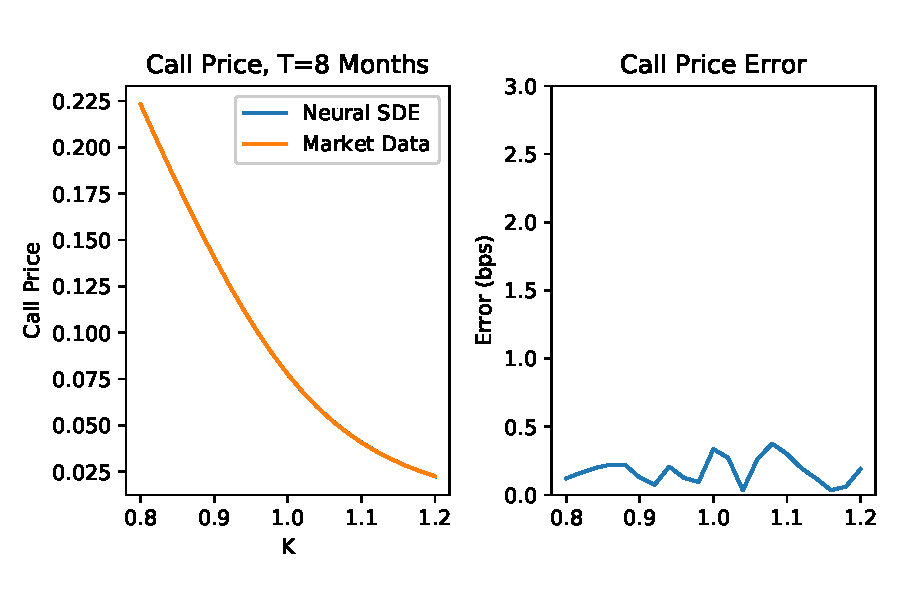
\includegraphics[clip,width=0.3\textwidth]{content/reschap1/Figures/figures_LV/Neural_SDE_maturity64_vanilla}
%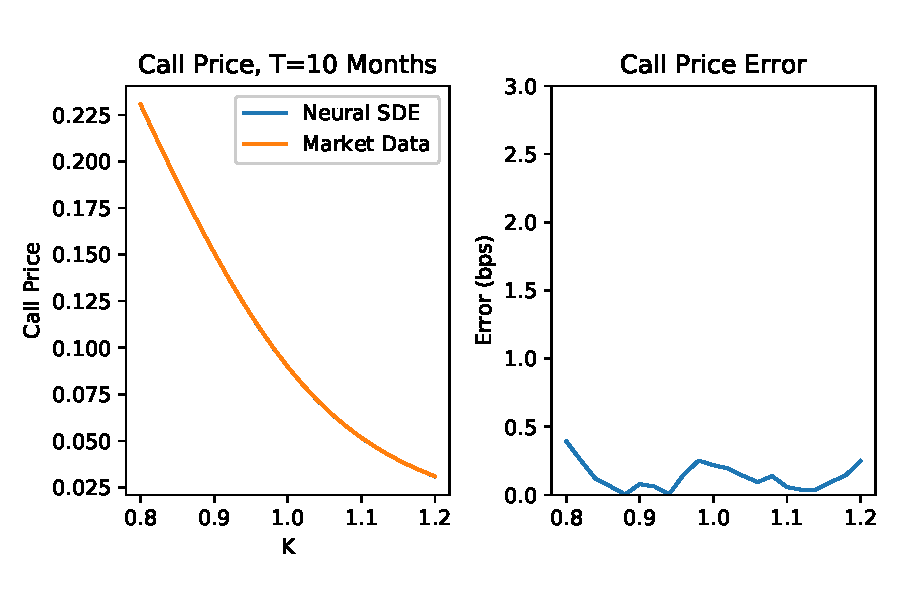
\includegraphics[clip,width=0.3\textwidth]{content/reschap1/Figures/figures_LV/Neural_SDE_maturity80_vanilla} 
%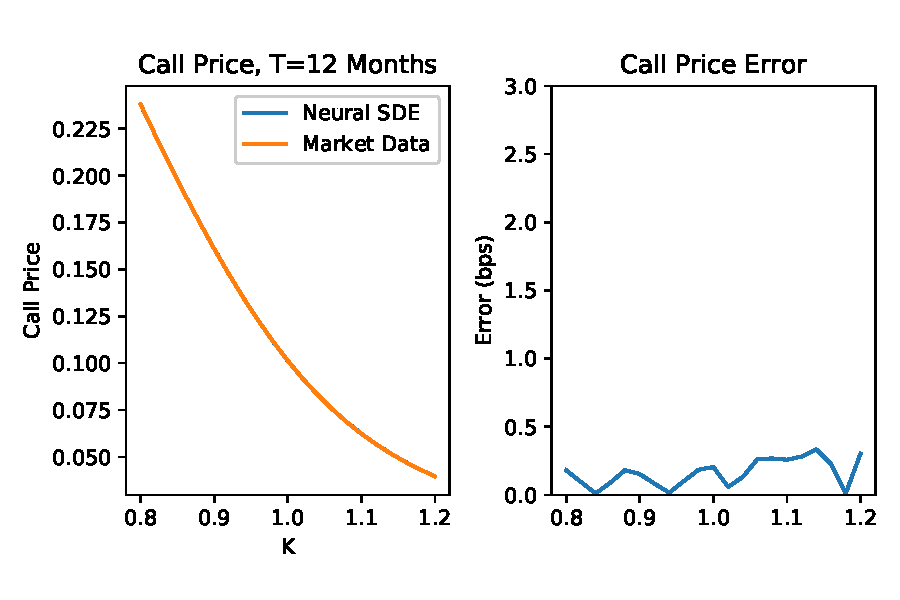
\includegraphics[clip,width=0.3\textwidth]{content/reschap1/Figures/figures_LV/Neural_SDE_maturity96_vanilla}
%\caption{Calibrated neural SDE LV model and market target prices comparison.}
%\label{FigUncprice}
%\end{figure}
%
%
%
%\begin{figure}[h]
%\centering 
%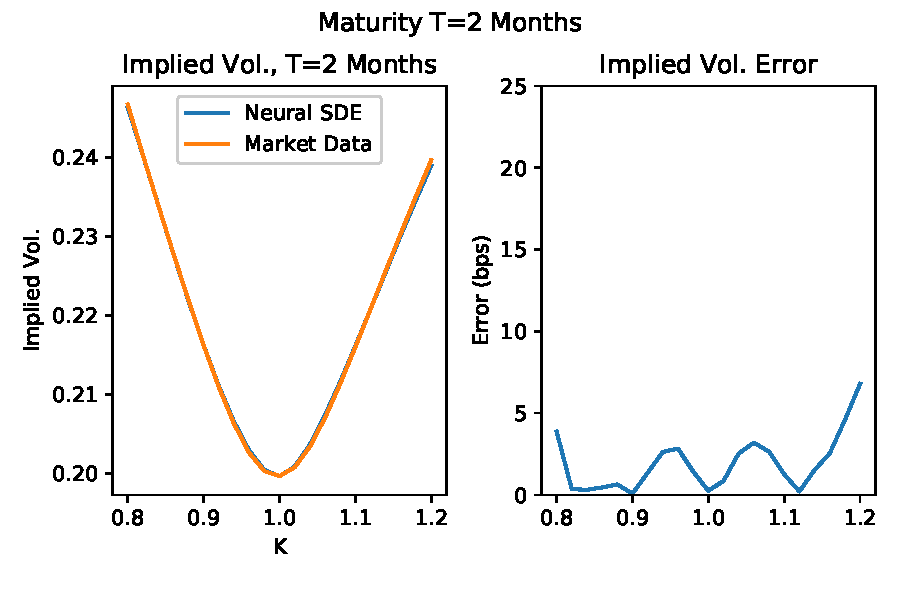
\includegraphics[clip,width=0.3\textwidth]{content/reschap1/Figures/figures_LV/Neural_SDE_lowerbound_maturity16_iv}
%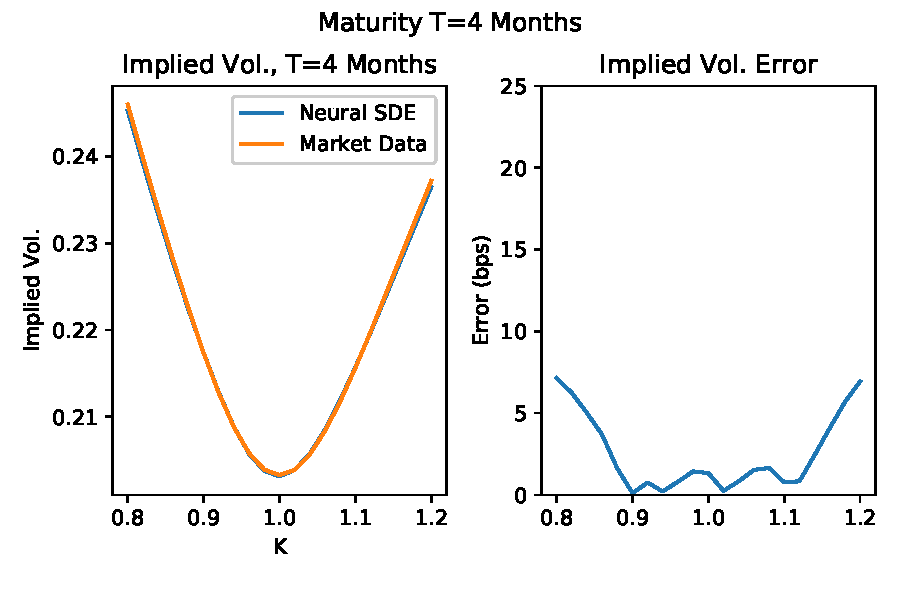
\includegraphics[clip,width=0.3\textwidth]{content/reschap1/Figures/figures_LV/Neural_SDE_lowerbound_maturity32_iv}
%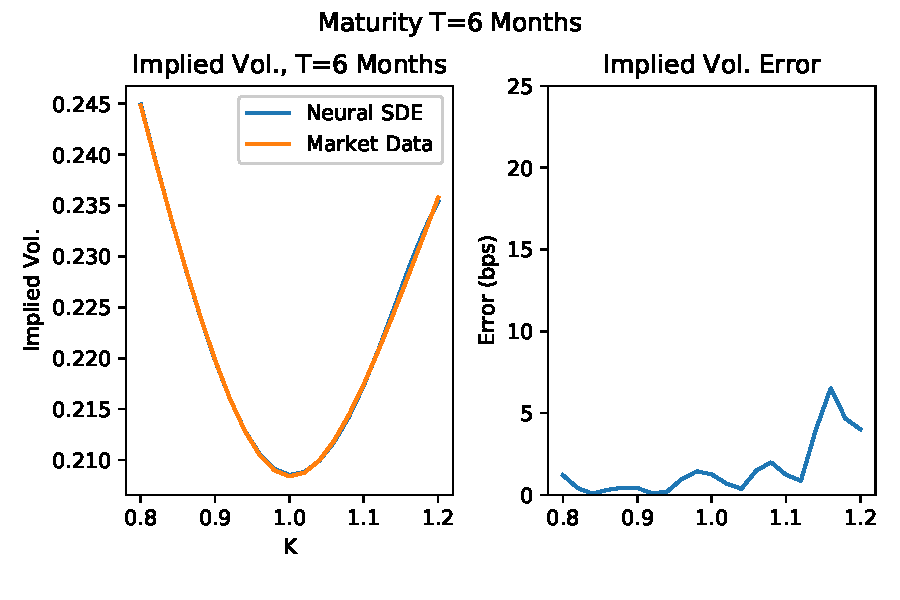
\includegraphics[clip,width=0.3\textwidth]{content/reschap1/Figures/figures_LV/Neural_SDE_lowerbound_maturity48_iv} 
%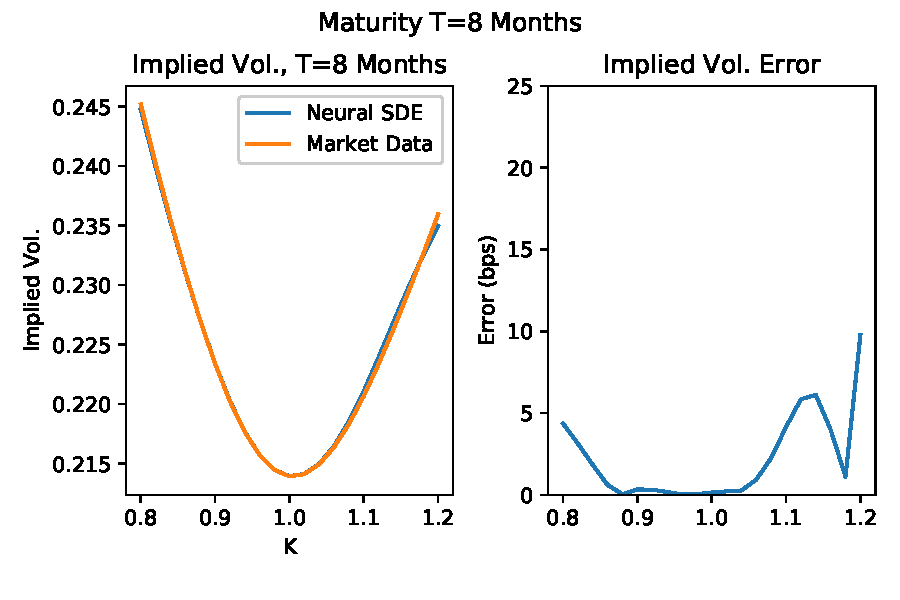
\includegraphics[clip,width=0.3\textwidth]{content/reschap1/Figures/figures_LV/Neural_SDE_lowerbound_maturity64_iv}
%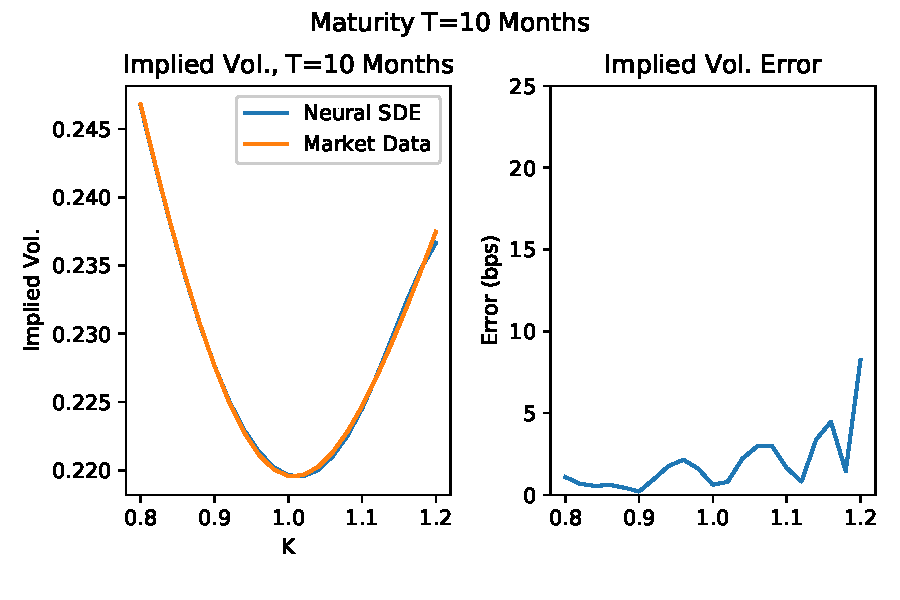
\includegraphics[clip,width=0.3\textwidth]{content/reschap1/Figures/figures_LV/Neural_SDE_lowerbound_maturity80_iv} 
%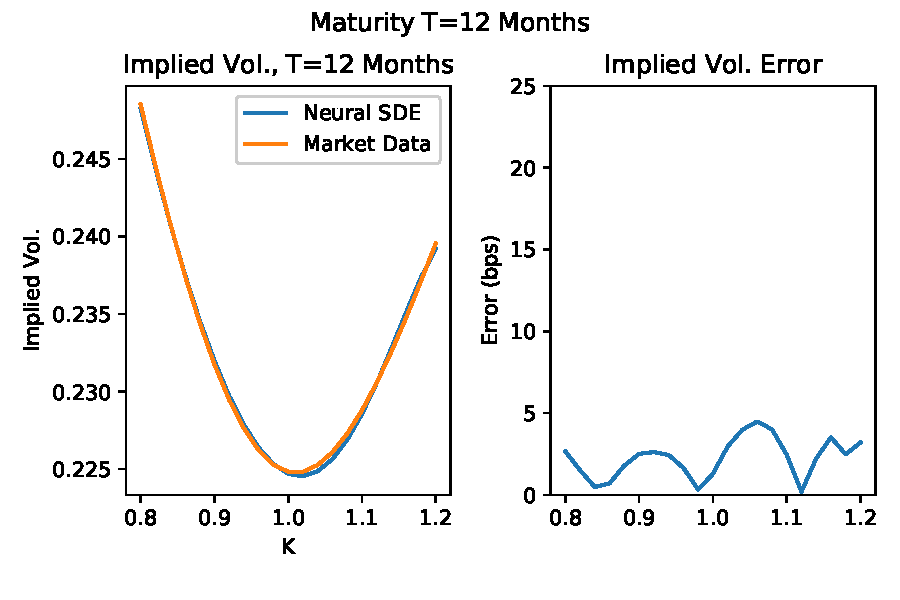
\includegraphics[clip,width=0.3\textwidth]{content/reschap1/Figures/figures_LV/Neural_SDE_lowerbound_maturity96_iv}
%\caption{Calibrated neural SDE LV model (with lower bound minimization on exotic payoff) and target market data implied volatility comparison.}
%\label{FigLB}  
%\end{figure}
%
%\begin{figure}[h]\label{FigLBprice}
%  \centering 
%  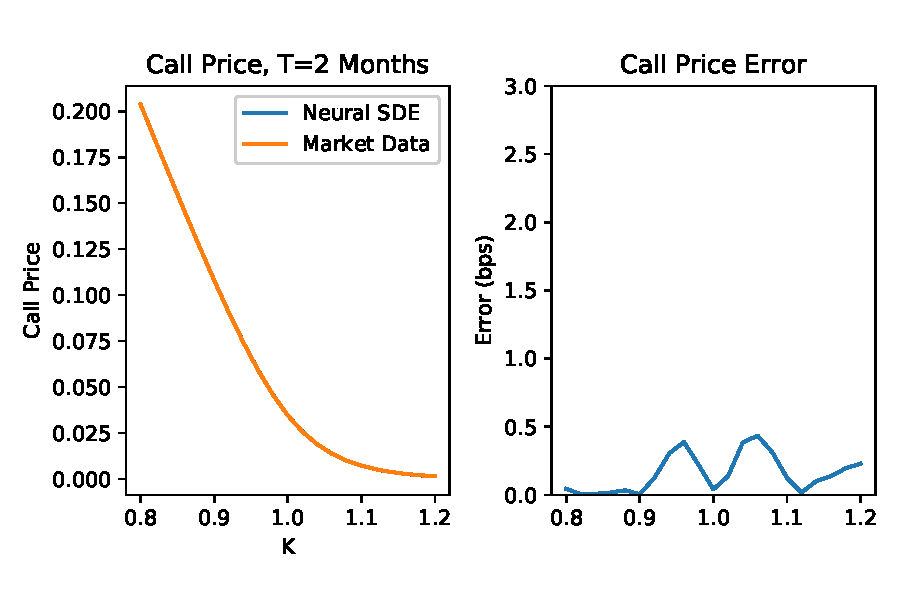
\includegraphics[clip,width=0.3\textwidth]{content/reschap1/Figures/figures_LV/Neural_SDE_lowerbound_maturity16_vanilla}
%  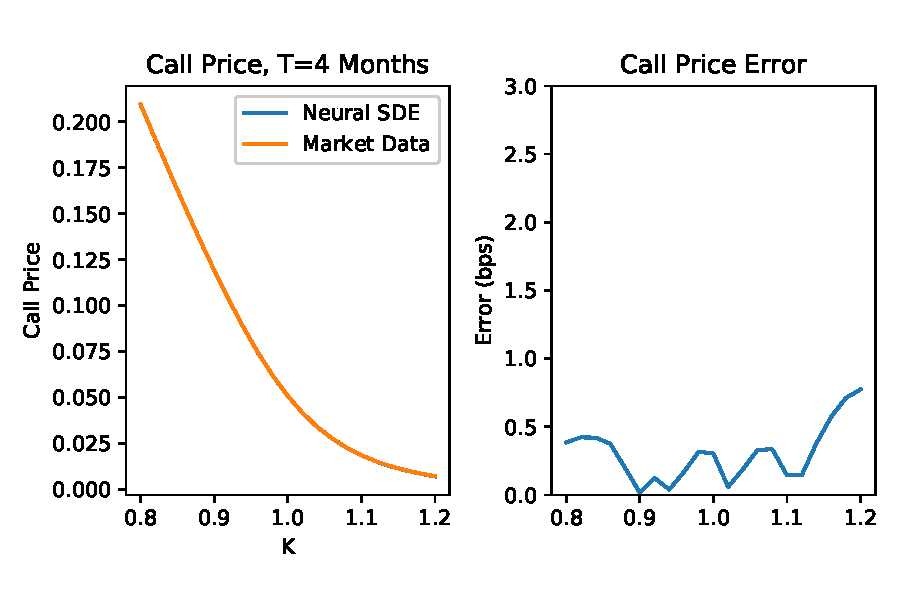
\includegraphics[clip,width=0.3\textwidth]{content/reschap1/Figures/figures_LV/Neural_SDE_lowerbound_maturity32_vanilla}
%  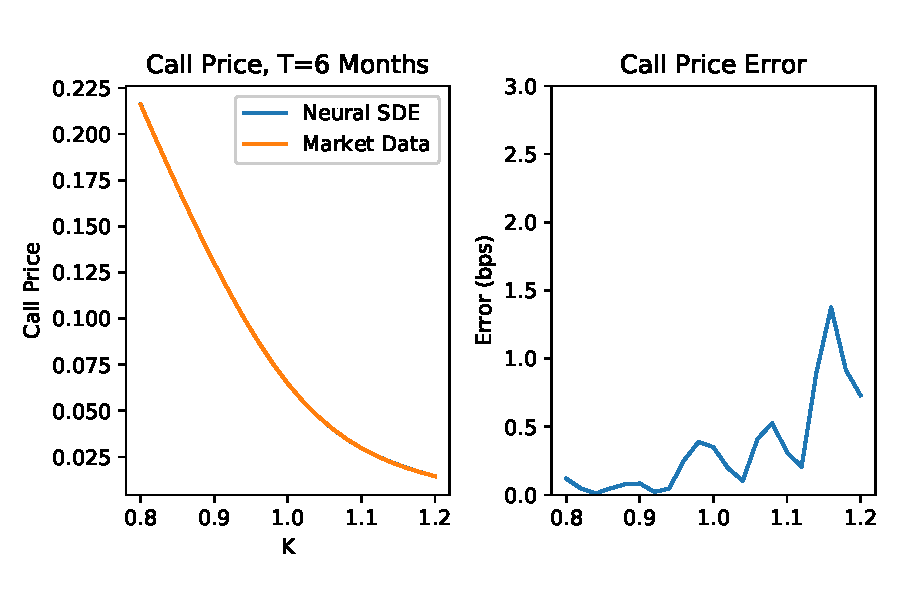
\includegraphics[clip,width=0.3\textwidth]{content/reschap1/Figures/figures_LV/Neural_SDE_lowerbound_maturity48_vanilla} 
%  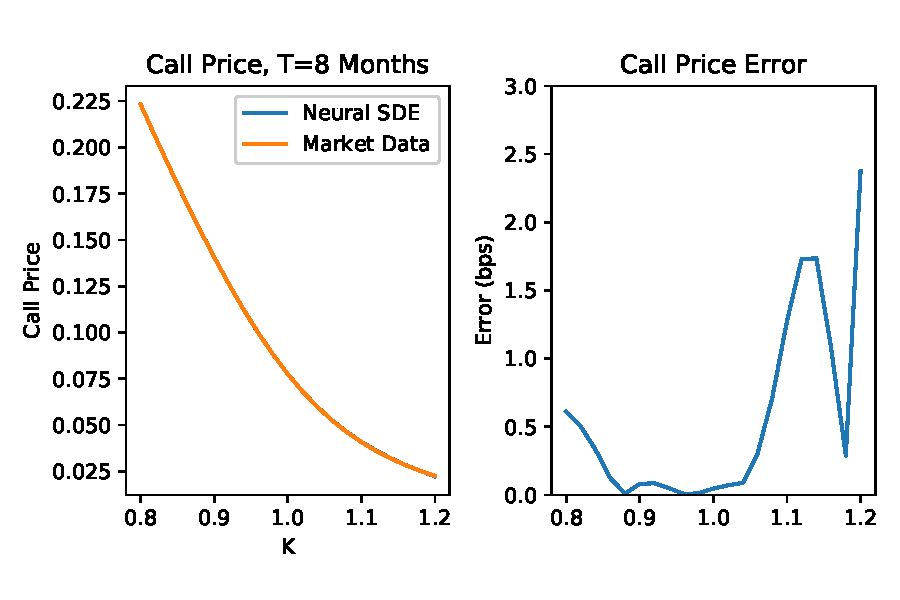
\includegraphics[clip,width=0.3\textwidth]{content/reschap1/Figures/figures_LV/Neural_SDE_lowerbound_maturity64_vanilla}
%  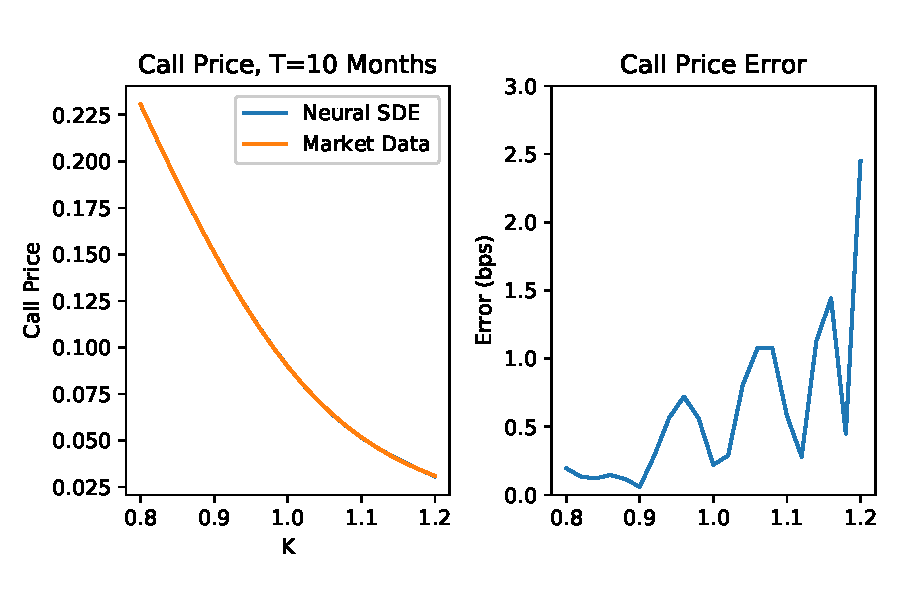
\includegraphics[clip,width=0.3\textwidth]{content/reschap1/Figures/figures_LV/Neural_SDE_lowerbound_maturity80_vanilla} 
%  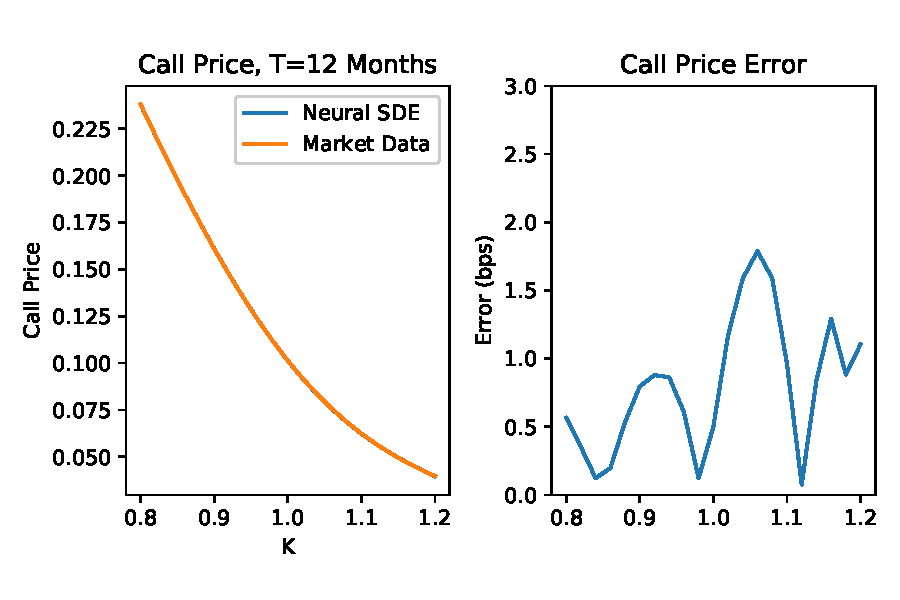
\includegraphics[clip,width=0.3\textwidth]{content/reschap1/Figures/figures_LV/Neural_SDE_lowerbound_maturity96_vanilla}
%  \caption{Calibrated neural SDE LV model (with lower bound minimization on exotic payoff) and target market prices comparison.}
%  \label{FigLBprice}
%\end{figure}
%
%
%\begin{figure}[h]\label{FigUB}
%\centering 
%\includegraphics[clip,width=0.3\textwidth]{content/reschap1/Figures/figures_LV/Neural_SDE_upperbound_maturity16_iv}
%  \includegraphics[clip,width=0.3\textwidth]{content/reschap1/Figures/figures_LV/Neural_SDE_upperbound_maturity32_iv}
%  \includegraphics[clip,width=0.3\textwidth]{content/reschap1/Figures/figures_LV/Neural_SDE_upperbound_maturity48_iv} 
%  \includegraphics[clip,width=0.3\textwidth]{content/reschap1/Figures/figures_LV/Neural_SDE_upperbound_maturity64_iv}
%  \includegraphics[clip,width=0.3\textwidth]{content/reschap1/Figures/figures_LV/Neural_SDE_upperbound_maturity80_iv} 
%  \includegraphics[clip,width=0.3\textwidth]{content/reschap1/Figures/figures_LV/Neural_SDE_upperbound_maturity96_iv}
%  \caption{Calibrated neural LV model (with upper bound maximization on exotic payoff) and target market data implied volatility comparison.}
% \label{FigUB}
%\end{figure}
%
%\begin{figure}[h]
%\centering 
%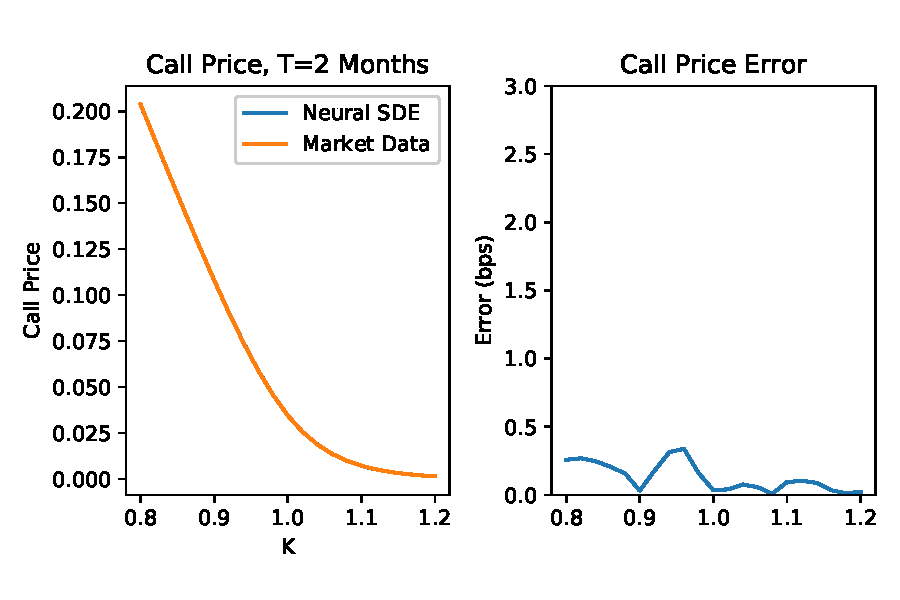
\includegraphics[clip,width=0.3\textwidth]{content/reschap1/Figures/figures_LV/Neural_SDE_maturity16_vanilla}
%  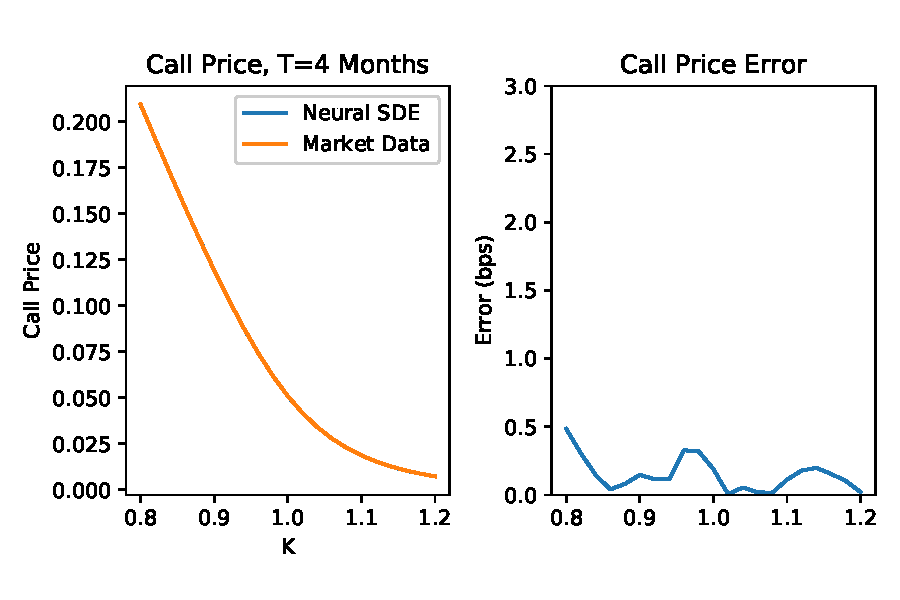
\includegraphics[clip,width=0.3\textwidth]{content/reschap1/Figures/figures_LV/Neural_SDE_maturity32_vanilla}
%  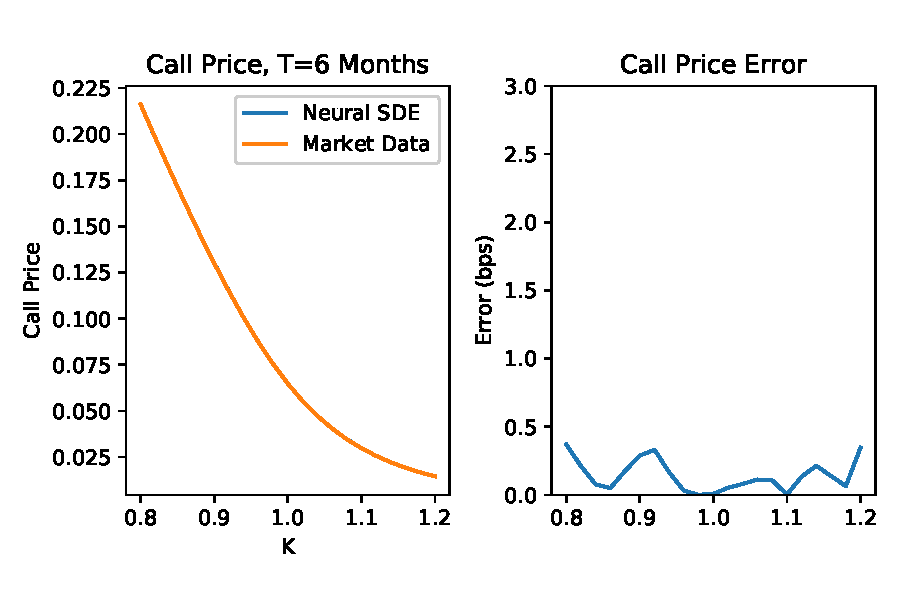
\includegraphics[clip,width=0.3\textwidth]{content/reschap1/Figures/figures_LV/Neural_SDE_maturity48_vanilla} 
%  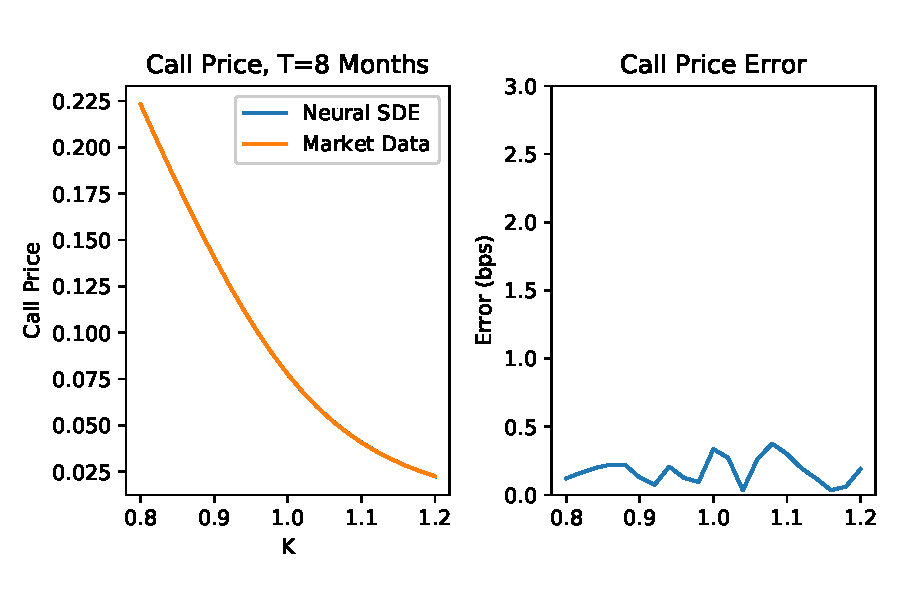
\includegraphics[clip,width=0.3\textwidth]{content/reschap1/Figures/figures_LV/Neural_SDE_maturity64_vanilla}
%  \includegraphics[clip,width=0.3\textwidth]{content/reschap1/Figures/figures_LV/Neural_SDE_maturity80_vanilla} 
%  \includegraphics[clip,width=0.3\textwidth]{content/reschap1/Figures/figures_LV/Neural_SDE_maturity96_vanilla}
%\caption{Calibrated LV neural model (with upper bound maximization on exotic payoff) and target market prices comparison.}
%\label{FigUBprice}
%\end{figure}
%
%\section{LSV neural SDEs calibration accuracy}
%\label{sec LSVfitquality}
%
%Figures~\ref{fig LSV calibration lb}, \ref{fig LSV calibration} and~\ref{fig LSV calibration ub} provide the Vanilla call option price and the implied volatility curve
%for the calibrated models. 
%In each plot, the blue line corresponds to the target data (generated using the Heston model), and each orange line corresponds to one run of the 
%neural SDE calibration. We note again in this plot how the absolute error of the calibration to the vanilla prices is consistently of~$\Oo(10^{-4})$.  
%
%
%
%\begin{figure}[h]
%  \centering 
%  \includegraphics[clip,width=0.3\textwidth]{content/reschap1/Figures/figures_LSV/lowerbound_64}
%  \includegraphics[clip,width=0.3\textwidth]{content/reschap1/Figures/figures_LSV/lowerbound_80}
%  \includegraphics[clip,width=0.3\textwidth]{content/reschap1/Figures/figures_LSV/lowerbound_96} 
%  \caption{Comparing market and model data fit for the neural SDE LSV model~\eqref{eq LSV SDE} when targeting the {\em lower bound} on the illiquid derivative. 
%We see vanilla option prices and implied volatility curves of the 10 calibrated neural SDEs vs. the market data for different maturities.
%}
%\label{fig LSV calibration lb}  
%\end{figure}
%
%
%
%
%\begin{figure}[h]
%  \centering 
%  \includegraphics[clip,width=0.3\textwidth]{content/reschap1/Figures/figures_LSV/upperbound_64}
%  \includegraphics[clip,width=0.3\textwidth]{content/reschap1/Figures/figures_LSV/upperbound_80}
%  \includegraphics[clip,width=0.3\textwidth]{content/reschap1/Figures/figures_LSV/upperbound_96} 
%  \caption{Comparing market and model data fit for the neural SDE LSV model~\eqref{eq LSV SDE} when targeting the {\em upper bound} on the illiquid derivative. 
%We see vanilla option prices and implied volatility curves of the 10 calibrated neural SDEs vs. the market data for different maturities.
%}
%\label{fig LSV calibration ub}
%\end{figure}



%\section{Exotic price in LV neural SDEs}\label{LVtables}
%
%Below we see how different random seeds, constrained optimization algorithms and a number of strikes used in the market data input affect the illiquid derivative price in the Local Volatility neural SDE model.
%
%\begin{figure}[h]
%  \centering 
%  \includegraphics[clip,width=0.45\textwidth]{content/reschap1/Figures/figures_LV/Strikes_6months}
%  \includegraphics[clip,width=0.45\textwidth]{content/reschap1/Figures/figures_LV/Strikes_12months}
%  \caption{Lookback exotic option price in lower, upper and unconstrained implied by perfectly calibrated LV neural SDE calibrated to a varying number of market options quotes.}
%\label{Strikechart} 
%\end{figure}
%
%
%\begin{table}[h]
%\begin{tabular}{|c|c||c|c|c|c|c|c|c|} 
%\hline 
%Initialisation & Calibration type & t=2/12 & t=4/12 & t=6/12 & t=8/12 & t=10/12 & t=1 \\ 
%\hline \hline
%1 & Unconstrained & .055 & .088 & .113 & .134 &  .159 &  .178  \\
%\hline 
%2 & Unconstrained & .056 &  .086 & .113 & .132 & .158 & .175  \\ 
%\hline 
%1 & LB Lag. mult. & .055 & .086 & .107 & .127 & .143 & .154 \\ 
%\hline
%2 & LB Lag. mult.& .055 & .084 & .098 & .113 & .125 & .139 \\ 
%\hline
%1 & UB Lag. mult.& .056 & .099 & .119  & .142 & .163 & .214 \\ 
%\hline
%2 & UB Lag. mult. & .059 & .101 & .131  & .156 & .208 & .220\\
%\hline
%1 & LB Augmented & .055 & .077 & .107 & .113 & .127 & .136 \\ 
%\hline
%2 & LB Augmented & .056 & .085 & .109 & .123 & .139 & .158 \\ 
%\hline
%1 & UB Augmented & .058 & .102 & .139 & .156 & .188 & .224 \\ 
%\hline
%2 & UB Augmented & .057 & .088 & .128  & .151 & .167 & .184 \\ 
%\hline
%- & Heston 400k paths & .058 & .087 & .111 & .133 & .154 & .174\\ 
%%\hline
%%- & Heston 10 mil paths & .058 & .087 & .111 & .133 & .154 & .174 \\ 
%%\hline
%%- & Local vol 400k paths & . & . & . & . & . & . \\ 
%%\hline
%%- & Local vol 10mil paths  & . & . & . & . & . & . \\ 
%\hline
%\end{tabular}
%\caption{Impact of initialisation and constrained optimization algorithms on prices of an illiquid derivative (lookback call) implied by LV neural SDE calibrated to vanilla prices with~$K=11$ strikes:~$k_1=0.9, k_2=0.92,...,k_{11}=1.1$ for each maturity.}
%\label{InitialisationImpact11strikes} 
%\end{table}  
%
%\begin{table}[h!tbp]
%\begin{tabular}{|c|c||c|c|c|c|c|c|c|} 
%\hline 
%Initialisation & Calibration type & t=2/12 & t=4/12 & t=6/12 & t=8/12 & t=10/12 & t=1 \\ 
%\hline \hline
%1 & Unconstrained & .056 & .087 & .114 & .140 & .161 & .182  \\
%\hline 
%2 & Unconstrained & .056 & .087 & .114 & .136 & .161 & .180  \\ 
%\hline 
%1 & LB Lag. mult. & .056 & .086 & .110 & .123 & .141 & .153 \\ 
%\hline
%2 & LB Lag. mult.& .056 & .087 & .108 & .125 &  .150 & .155 \\ 
%\hline
%1 & UB Lag. mult.& .056 & .088 & .120  & .156 & .179 & .205 \\ 
%\hline
%2 & UB Lag. mult. & .056 & .088 & .118  & .153 & .187 & .208\\
%\hline
%1 & LB Augmented & .056 & .087 & .108 & .128 & .143 & .164 \\ 
%\hline
%2 & LB Augmented & .056 & .087 & .108 & .125 & .150 & .155 \\ 
%\hline
%1 & UB Augmented & .056 & .091 & .124 & .155 & .173 & .194\\ 
%\hline
%2 & UB Augmented & .056 & .088 & .125 & .146 & .167 &  .189\\ 
%\hline
%- & Heston 400k paths & .058 & .087 & .111 & .133 & .154 & .174 \\ 
%\hline
%- & Heston 10mil paths & .058 & .087 & .111 & .133 & .154 & .174 \\ 
%%\hline
%%- & Local vol 400k paths & . & . & . & . & . & . \\ 
%%\hline
%%- & Local vol 10mil paths  & . & . & . & . & . & . \\ 
%\hline
%\end{tabular}
%\caption{Impact of initialisation Prices of ATM lookback call implied by LV neural SDE calibrated to vanilla prices with~$K=21$ strikes:~$k_1=0.8, k_2=0.82,...,k_{21}=1.2$ for each maturity.}
%\label{InitialisationImpact21strikes} 
%\end{table}  
%
%
%\begin{table}[h!tbp]
%\begin{tabular}{|c|c||c|c|c|c|c|c|c|} 
%\hline 
%Initialisation & Calibration type & t=2/12 & t=4/12 & t=6/12 & t=8/12 & t=10/12 & t=1 \\ 
%\hline \hline
%1 & Unconstrained & .056 & .087 & .114 & .138 &  .162 &  .184  \\
%\hline 
%2 & Unconstrained & .056 &  .087 & .114 & .138 & .160 & .183  \\ 
%\hline 
%1 & LB Lag. mult. & .056 & .087 & .113 & .137 & .149 & .172 \\ 
%\hline
%2 & LB Lag. mult.& .056 & .087 & .113 & .136 & .155 & .165 \\ 
%\hline
%1 & UB Lag. mult.& .056 & .088 & .115  & .148 & .170 & .197 \\ 
%\hline
%2 & UB Lag. mult. & .056 & .087 & .114  & .144 & .170 & .198\\
%\hline
%1 & LB Augmented & .056 & .087 & .114 & .138 & .161 & .183 \\ 
%\hline
%2 & LB Augmented & .056 & .087 & .112 & .130 & .154 & .166 \\ 
%\hline
%1 & UB Augmented & .056 & .087 & .114 & .138 & .162 & .183 \\ 
%\hline
%2 & UB Augmented & .056 & .087 & .114 & .141 & .164 & .190 \\ 
%\hline
%- & Heston 400k paths& .058 & .087 & .111 & .133 & .154 & .174 \\ 
%\hline
%- & Heston 10mil paths & .058 & .087 & .111 & .133 & .154 & .174 \\ 
%%\hline
%%- & Local vol 400k paths & . & . & . & . & . & . \\ 
%%\hline
%%- & Local vol 10mil paths  & . & . & . & . & . & . \\ 
%\hline
%\end{tabular}
%\caption{Impact of initialisation Prices of ATM lookback call implied by LV neural SDE calibrated to vanilla prices with~$K=31$ strikes:~$k_1=0.7, k_2=0.72,...,k_{31}=1.3$ for each maturity.}
%\label{InitialisationImpact31strikes} 
%\end{table}  
%
%\begin{table}[h!tbp]
%\begin{tabular}{|c|c||c|c|c|c|c|c|c|} 
%\hline 
%Initialisation & Calibration type & t=2/12 & t=4/12 & t=6/12 & t=8/12 & t=10/12 & t=1 \\ 
%\hline \hline
%1 & Unconstrained & .056 & .087 & .114 & .138 &  .160 &  .183  \\
%\hline 
%2 & Unconstrained & .056 &  .087 & .113 & .138 & .162 & .184  \\ 
%\hline 
%1 & LB Lag. mult. & .056 & .087 & .113 & .137 & .158 & .172 \\ 
%\hline
%2 & LB Lag. mult.& .056 & .087 & .113 & .137 & .153 & .171 \\ 
%\hline
%1 & UB Lag. mult.& .056 & .088 & .117  & .141 & .166 & .193 \\ 
%\hline
%2 & UB Lag. mult. & .056 & .087 & .116  & .140 & .166 & .192 \\
%\hline
%1 & LB Augmented & .056 & .087 & .113 & .136 & .153 & .172 \\ 
%\hline
%2 & LB Augmented & .056 & .087 & .113 & .136 & .152 & .169 \\ 
%\hline
%1 & UB Augmented & .056 & .087 & .114 & .138 & .160 & .182 \\ 
%\hline
%2 & UB Augmented & .056 & .087 & .116 & .140 & .164 & .191 \\ 
%\hline
%- & Heston 400k paths & .058 & .087 & .111 & .133 & .154 & .174 \\ 
%\hline
%- & Heston 10mil paths & .058 & .087 & .111 & .133 & .154 & .174 \\ 
%%\hline
%%- & Local vol 400kpaths & . & . & . & . & . & . \\ 
%%\hline
%%- & Local vol 10mil paths  & . & . & . & . & . & . \\ 
%\hline
%\end{tabular}
%
%\caption{Impact of initialisation Prices of ATM lookback call implied by LV neural SDE calibrated to vanilla prices with~$K=41$ strikes:~$k_1=0.6, k_2=0.62,...,k_{41}=1.4$ for each maturity.}
%\label{InitialisationImpact41strikes} 
%\end{table}  
%
